\section{Casi d'uso}
Di seguito verranno illustrati i casi d'uso\glossario{} individuati per il progetto \project{}.
Ogni caso d'uso\glossario{} avrà un codice identificativo di forma:
\begin{center}
UC[codice univoco del padre].[codice progressivo di livello].
\end{center}
Il codice progressivo di livello può includere diversi livelli di gerarchia separati da un punto. Lo scenario principale sarà comunque individuato attraverso il codice UCP e successivamente verranno descritti i figli, senza però individuare nel loro codice il padre.

\subsection{Caso d'uso UCP: Scenario principale}

\begin{figure}[!h]
\begin{center}
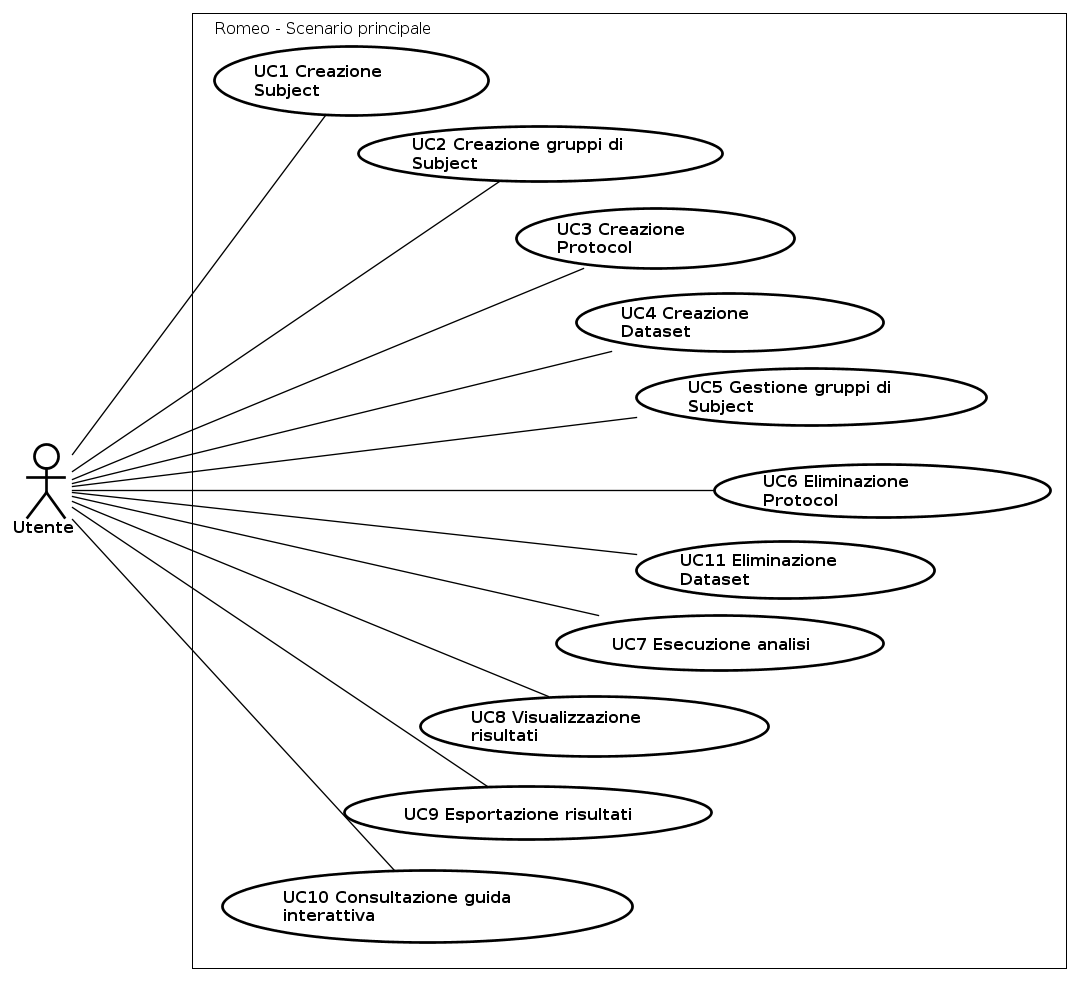
\includegraphics[scale=0.5]{./img/Use_Case/UCP}
\caption{UCP - Scenario principale}
\end{center}
\end{figure}

\begin{itemize}
\item \textbf{Attori:} Utente;
\item \textbf{Scopo e descrizione:} l'utente, dopo aver avviato il software, può effettuare diverse operazioni. Egli può creare singolarmente: Subject\glossario{}, gruppi di Subject\glossario{}, Protocol\glossario{} e Dataset\glossario{}. Se già presenti, può eliminare Protocol\glossario{} e gruppi di Subject\glossario{}; inoltre se è presente almeno un Dataset\glossario{}, può eseguire l'analisi di quel Dataset\glossario{} e se ha già effettuato un'analisi, può visualizzarne i risultati e/o esportarli. Infine può consultare la guida interattiva;
\item \textbf{Precondizione:} il programma è stato avviato ed è pronto all'uso;
\item \textbf{Flusso principale degli eventi:} 
\begin{enumerate}
\item l'utente può creare dei Subject\glossario{} [UC1];
\item l'utente può creare un gruppo di Subject\glossario{} [UC2];
\item l'utente può creare un Protocol\glossario{} [UC3];
\item l'utente può creare un Dataset\glossario{} [UC4];
\item l'utente può gestire un gruppo di Subject\glossario{} [UC5];
\item l'utente può eliminare un Protocol\glossario{} [UC6];
\item l'utente può eseguire un'analisi [UC7];
\item l'utente può visualizzare i risultati di un'analisi [UC8];
\item l'utente può esportare i risultati di un'analisi [UC9];
\item l'utente può consultare la guida interattiva [UC10].
\item l'utente può eliminare un \dataset{} [UC11];
\end{enumerate}
\item \textbf{Postcondizione:} il programma ha ottenuto le informazioni delle operazioni che l'utente desidera effettuare.
\end{itemize}

\subsection{Caso d'uso UC1: Creazione Subject}
\begin{figure}[!h]
\begin{center}
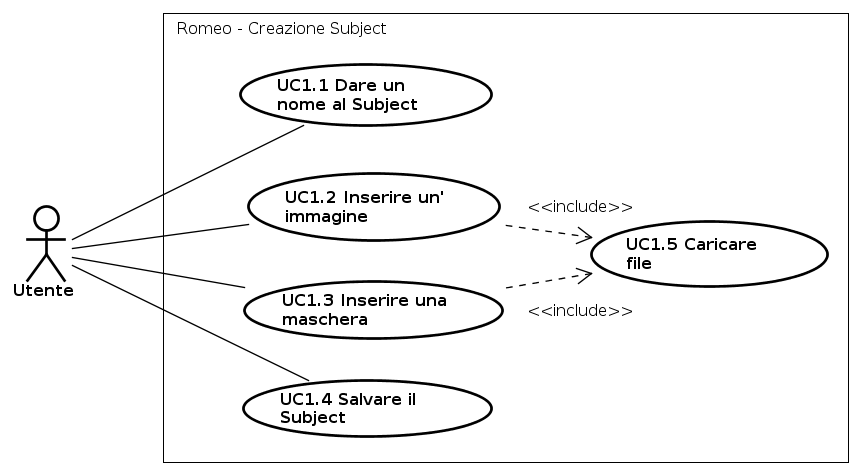
\includegraphics[scale=0.6]{./img/Use_Case/UC1}
\caption{UC1 - Creazione Subject}
\end{center}
\end{figure}
\begin{itemize}
\item \textbf{Attori:} Utente;
\item \textbf{Scopo e descrizione:} l'utente sta creando un Subject\glossario{}. Per completare l'operazione, deve assegnargli un nome, inserire un'immagine ed eventualmente associargli una maschera\glossario{};
\item \textbf{Precondizione:} il sistema mostra la schermata di creazione Subject\glossario{} e l'utente vuole creare un Subject\glossario{};
\item \textbf{Flusso principale degli eventi:} 
\begin{enumerate}
\item l'utente deve dare un nome al Subject\glossario{} [UC1.1];
\item l'utente deve inserire un'immagine [UC1.2];
\item l'utente carica un file per inserire l'immagine [UC1.5];
\item l'utente può inserire una maschera\glossario{} [UC1.3];
\item l'utente carica un file per inserire la maschera\glossario{} [UC1.5];
\item l'utente conferma il Subject\glossario{} appena creato [UC1.4].
\end{enumerate}
\item \textbf{Scenario alternativo:} l'utente inserisce un nome già precedentemente usato per un altro Subject\glossario{}. Il sistema segnala il conflitto e chiede di inserire un nome non ancora usato;
\item \textbf{Postcondizione:} il sistema ha memorizzato il Subject\glossario{} creato dall'utente.
\end{itemize}

\subsection{Caso d'uso UC1.1: Dare un nome al Subject}
\begin{itemize}
\item \textbf{Attori:} Utente;
\item \textbf{Scopo e descrizione:} l'utente deve dare un nome al Subject\glossario{} che sta creando per essere in grado di identificarlo successivamente;
\item \textbf{Precondizione:} il sistema è in attesa che l'utente inserisca il nome del Subject\glossario{};
\item \textbf{Flusso principale degli eventi:}
\begin{enumerate}
\item l'utente deve dare un nome univoco al \subject{}.
\end{enumerate}
\item \textbf{Postcondizione:} il sistema associa al Subject\glossario{} in creazione, il nome inserito dall'utente.
\end{itemize}

\subsection{Caso d'uso UC1.2: Inserire un'immagine}
\begin{itemize}
\item \textbf{Attori:} Utente;
\item \textbf{Scopo e descrizione:} l'utente deve inserire l'immagine che desidera associare al Subject\glossario{};
\item \textbf{Precondizione:} il sistema è in attesa che l'utente selezioni l'immagine;
\item \textbf{Flusso principale degli eventi:}
\begin{enumerate}
\item l'utente inserisce un'immagine per il \subject{}.
\end{enumerate}
\item \textbf{Postcondizione:} il sistema ha caricato l'immagine e l'ha associata al Subject\glossario{}.
\end{itemize}

\subsection{Caso d'uso UC1.3: Inserire una maschera}
\begin{itemize}
\item \textbf{Attori:} Utente;
\item \textbf{Scopo e descrizione:} l'utente inserisce una maschera\glossario{} per limitare l'area di analisi dell'immagine;
\item \textbf{Precondizione:} il sistema mostra la schermata di creazione del Subject\glossario{} e l'utente ha deciso di caricare una maschera\glossario{};
\item \textbf{Flusso principale degli eventi:}
\begin{enumerate}
\item l'utente inserisce una maschera\glossario{} per il \subject{}.
\end{enumerate}
\item \textbf{Postcondizione:} il sistema ha caricato la maschera\glossario{} e l'ha associata al Subject\glossario{}.
\end{itemize}

\subsection{Caso d'uso UC1.4: Salvare il Subject}
\begin{itemize}
\item \textbf{Attori:} Utente;
\item \textbf{Scopo e descrizione:} l'utente salva il Subject\glossario{} appena creato;
\item \textbf{Precondizione:} l'utente ha inserito un nome esatto e un'immagine;
\item \textbf{Flusso principale degli eventi:}
\begin{enumerate}
\item l'utente salva il \subject{}.
\end{enumerate}
\item \textbf{Postcondizione:} il sistema ha salvato il Subject\glossario{} appena creato dall'utente.
\end{itemize}

\subsection{Caso d'uso UC1.5: Caricare file}
\begin{figure}[!h]
\begin{center}
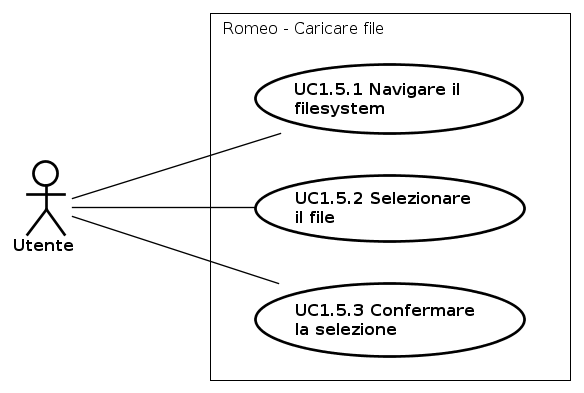
\includegraphics[scale=0.6]{./img/Use_Case/UC1_5}
\caption{UC1.5 - Caricare file}
\end{center}
\end{figure}
\begin{itemize}
\item \textbf{Attori:} Utente;
\item \textbf{Scopo e descrizione:} l'utente deve caricare un file, l'immagine o la maschera\glossario{} del Subject\glossario{}. Egli naviga il filesystem alla ricerca del file desiderato, lo seleziona e conferma la selezione caricando il file;
\item \textbf{Precondizione:} l'utente ha scelto di inserire l'immagine del \subject{} o la sua maschera\glossario{}, il sistema attende l'input dell'utente;
\item \textbf{Flusso principale degli eventi:}
\begin{enumerate}
\item l'utente naviga il filesystem alla ricerca del file desiderato [UC1.5.1];
\item l'utente seleziona il file [UC1.5.2];
\item l'utente conferma il file selezionato [UC1.5.3].
\end{enumerate}
\item \textbf{Scenario alternativo:} l'utente interrompe la selezione del file e il sistema torna allo stato precedente l'inizio della selezione;
\item \textbf{Postcondizione:} il sistema ha caricato il file selezionato dall'utente e l'ha associato al Subject\glossario{}.
\end{itemize}

\subsection{Caso d'uso UC1.5.1: Navigare il filesystem}
\begin{itemize}
\item \textbf{Attori:} Utente;
\item \textbf{Scopo e descrizione:} l'utente può navigare il filesystem per selezionare la cartella dove è contenuto il file che vuole caricare;
\item \textbf{Precondizione:} il sistema è in attesa che l'utente selezioni una cartella;
\item \textbf{Flusso principale degli eventi:}
\begin{enumerate}
\item l'utente naviga nel filesystem alla ricerca del file desiderato.
\end{enumerate}
\item \textbf{Postcondizione:} il sistema ha aggiornato la cartella corrente con quella indicata dall'utente.
\end{itemize}

\subsection{Caso d'uso UC1.5.2 Selezionare il file}
\begin{itemize}
\item \textbf{Attori:} Utente;
\item \textbf{Scopo e descrizione:} l'utente deve selezionare il file che desidera caricare;
\item \textbf{Precondizione:} il sistema mostra i file che sono contenuti nella cartella precedentemente selezionata;
\item \textbf{Flusso principale degli eventi:}
\begin{enumerate}
\item l'utente seleziona il file che desidera caricare.
\end{enumerate}
\item \textbf{Postcondizione:} il sistema evidenzia il file che l'utente ha indicato.
\end{itemize}

\subsection{Caso d'uso UC1.5.3: Confermare la selezione}
\begin{itemize}
\item \textbf{Attori:} Utente;
\item \textbf{Scopo e descrizione:} l'utente conferma che il file selezionato precedentemente è quello che desidera caricare;
\item \textbf{Precondizione:} il sistema ha selezionato il file indicato dall'utente;
\item \textbf{Flusso principale degli eventi:}
\begin{enumerate}
\item l'utente conferma il file selezionato precedentemente.
\end{enumerate}
\item \textbf{Postcondizione:} il sistema ha caricato il file precedentemente indicato dall'utente.
\end{itemize}


\subsection{Caso d'uso UC2: Creazione di un gruppo di Subject}
\begin{figure}[!h]
\begin{center}
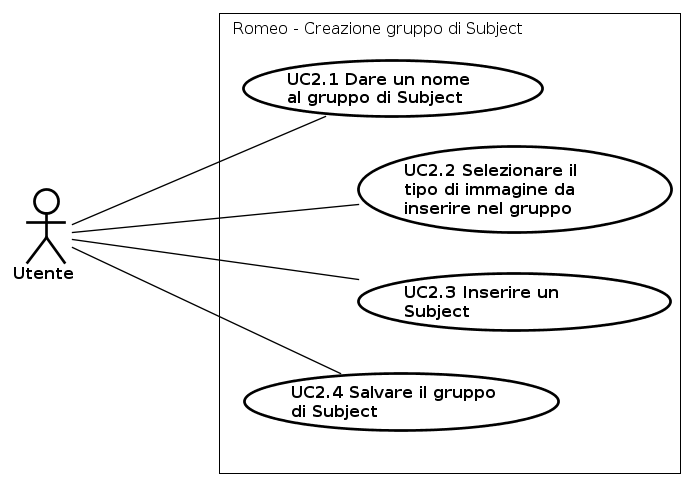
\includegraphics[scale=0.6]{./img/Use_Case/UC2}
\caption{UC2 - Creazione di un gruppo di Subject}
\end{center}
\end{figure}
\begin{itemize}
\item \textbf{Attori:} Utente;
\item \textbf{Scopo e descrizione:} l'utente vuole creare un gruppo di Subject\glossario{}. Come prima cosa, deve assegnare un nome al gruppo e selezionare il tipo dei Subject\glossario{} che ne faranno parte (2D, 2D-t, 3D o 3D-t). Successivamente, deve inserire i Subject\glossario{}, infine deve salvare il gruppo;
\item \textbf{Precondizione:} il sistema mostra la schermata di creazione dei gruppi di Subject\glossario{}; deve esserci almeno un Subject\glossario{} all'interno del sistema e l'utente deve aver scelto di creare un gruppo di Subject\glossario{};
\item \textbf{Flusso principale degli eventi:}
\begin{enumerate}
\item l'utente dà un nome al gruppo [UC2.1];
\item l'utente seleziona il tipo di immagine che i Subject\glossario{} del gruppo dovranno avere [UC2.2];
\item l'utente inserisce il singolo Subject\glossario{} [UC2.3];
\item l'utente salva il gruppo [UC2.4].
\end{enumerate}
\item \textbf{Scenario alternativo:} l'utente inserisce un nome già usato per un altro gruppo di Subject\glossario{}; il sistema segnala l'incongruenza e chiede di inserire un nome diverso;
\item \textbf{Postcondizione:} il sistema ha al suo interno il gruppo di Subject\glossario{} appena costruito.
\end{itemize}

\subsection{Caso d'uso UC2.1: Dare un nome al gruppo di Subject}
\begin{itemize}
\item \textbf{Attori:} Utente;
\item \textbf{Scopo e descrizione:} l'utente deve assegnare un nome al gruppo di Subject\glossario{} che sta creando, per poterlo successivamente identificare;
\item \textbf{Precondizione:} il sistema è in attesa che l'utente inserisca il nome del gruppo di Subject\glossario{};
\item \textbf{Flusso principale degli eventi:}
\begin{enumerate}
\item l'utente dà un nome al gruppo di \subject{}.
\end{enumerate}
\item \textbf{Postcondizione:} il sistema associa al gruppo di Subject\glossario{} in creazione, il nome inserito dall'utente.
\end{itemize}

\subsection{Caso d'uso UC2.2: Selezionare il tipo di immagine da inserire nel gruppo}
\begin{itemize}
\item \textbf{Attori:} Utente;
\item \textbf{Scopo e descrizione:} l'utente deve selezionare il tipo di immagine che vuole inserire nei Subject\glossario{} che saranno contenuti nel gruppo che sta creando. I tipi sono 2D, 2D-t, 3D e 3D-t;
\item \textbf{Precondizione:} il sistema è in attesa della scelta da parte dell'utente;
\item \textbf{Flusso principale degli eventi:}
\begin{enumerate}
\item l'utente seleziona il tipo di immagine da inserire nel gruppo.
\end{enumerate}
\item \textbf{Postcondizione:} il sistema conosce il tipo delle immagini che può accettare per questo gruppo di Subject\glossario{}.
\end{itemize}

\subsection{Caso d'uso UC2.3: Inserire un Subject}
\begin{itemize}
\item \textbf{Attori:} Utente;
\item \textbf{Scopo e descrizione:} l'utente deve inserire dei Subject\glossario{} all'interno di un gruppo e li deve scegliere tra quelli proposti dal sistema;
\item \textbf{Precondizione:} il sistema mostra la schermata di creazione Subject\glossario{}, assieme ad una lista di Subject\glossario{} contenenti immagini compatibili con il tipo selezionato dall'utente;
\item \textbf{Flusso principale degli eventi:}
\begin{enumerate}
\item l'utente inserisce un Subject\glossario{} nel gruppo.
\end{enumerate}
\item \textbf{Postcondizione:} il sistema ha inserito nel gruppo i Subject\glossario{} selezionati dall'utente.
\end{itemize}

\subsection{Caso d'uso UC2.4: Salvare il gruppo di Subject}
\begin{itemize}
\item \textbf{Attori:} Utente;
\item \textbf{Scopo e descrizione:} al termine della creazione, l'utente deve salvare il gruppo di Subject\glossario{};
\item \textbf{Precondizione:} il sistema mostra la schermata di creazione dei gruppi di Subject\glossario{} e l'utente ha inserito almeno un Subject\glossario{};
\item \textbf{Flusso principale degli eventi:}
\begin{enumerate}
\item l'utente salva il gruppo di Subject\glossario{}.
\end{enumerate}
\item \textbf{Postcondizione:} il sistema ha memorizzato il gruppo di Subject\glossario{} creato dall'utente.
\end{itemize}


\subsection{Caso d'uso UC3: Creazione Protocol}
\begin{figure}[!h]
\begin{center}
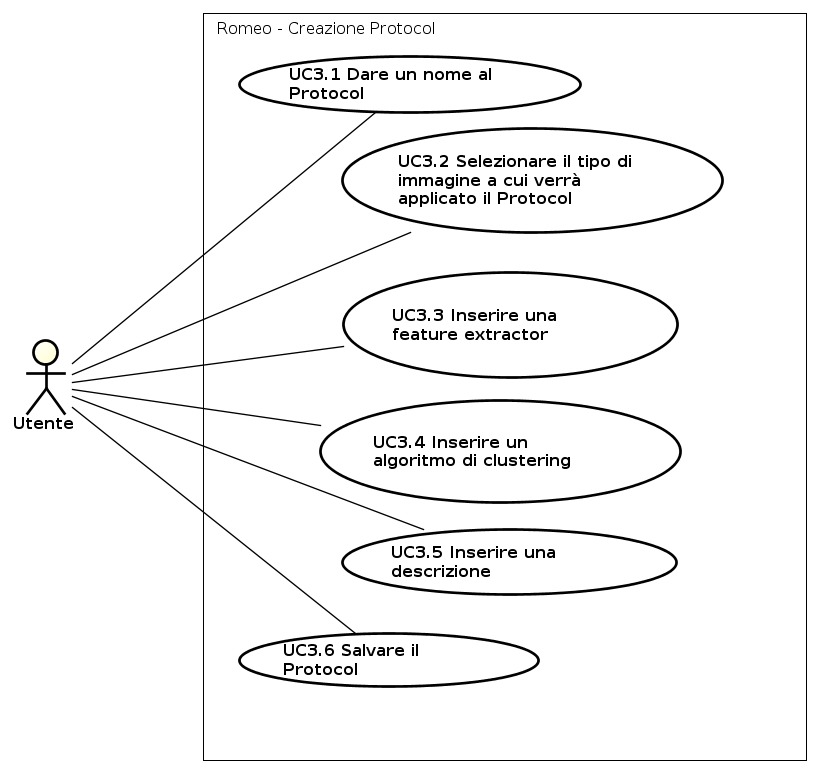
\includegraphics[scale=0.6]{./img/Use_Case/UC3}
\caption{UC3 - Creazione Protocol}
\end{center}
\end{figure}
\begin{itemize}
\item \textbf{Attori:} Utente;
\item \textbf{Scopo e descrizione:} l'utente ha scelto di creare un Protocol\glossario{} e in primo luogo deve assegnargli un nome. Successivamente, dato che un Protocol\glossario{} è composto da [0..N] feature extractors\glossario{} e da [0,1] algoritmi di clustering\glossario{}, l'utente deve scegliere la combinazione di funzioni che vuole utilizzare. Per questo, deve selezionare le feature extractors\glossario{} eventualmente scelte ed impostarne i parametri. Stesso procedimento va fatto per l'eventuale algoritmo di clustering\glossario{}. In secondo luogo, l'utente può inserire una breve descrizione riguardante il Protocol\glossario{}. Infine deve salvare il Protocol\glossario{} che ha appena creato;
\item \textbf{Precondizione:} il sistema mostra la schermata di creazione Protocol\glossario{}, fornendo una lista di feature extractors\glossario{} e algoritmi di clustering\glossario{} e l'utente ha scelto di creare un Protocol\glossario{};
\item \textbf{Flusso principale degli eventi:}
\begin{enumerate}
\item l'utente dà un nome al Protocol\glossario{} [UC3.1];
\item l'utente seleziona il tipo di immagini a cui avverrà applicato il Protocol\glossario{} [UC3.2];
\item l'utente inserisce o meno delle feature extractors\glossario{} [UC3.3];
\item l'utente inserisce o meno un algoritmo di clustering\glossario{} [UC3.4];
\item l'utente inserisce una descrizione testuale riguardante il Protocol\glossario{} [UC3.5];
\item l'utente salva il Protocol\glossario{} appena creato [UC3.6].
\end{enumerate}

\item \textbf{Scenario alternativo:} l'utente inserisce un nome già utilizzato per un precedente Protocol\glossario{}; il sistema segnala l'incompatibilità e chiede di inserire un nome diverso;
\item \textbf{Postcondizione:} il sistema ha memorizzato il Protocol\glossario{} appena creato dall'utente.
\end{itemize}

\subsection{Caso d'uso UC3.1: Dare un nome al Protocol}
\begin{itemize}
\item \textbf{Attori:} Utente;
\item \textbf{Scopo e descrizione:} l'utente deve dare un nome al Protocol\glossario{} che sta creando per poterlo successivamente identificare;
\item \textbf{Precondizione:} il sistema è in attesa che l'utente inserisca il nome del Protocol\glossario{};
\item \textbf{Flusso principale degli eventi:}
\begin{enumerate}
\item l'utente dà un nome al Protocol\glossario{}.
\end{enumerate}
\item \textbf{Postcondizione:} il sistema associa al Protocol\glossario{} in creazione, il nome inserito dall'utente.
\end{itemize}

\subsection{Caso d'uso UC3.2: Selezionare il tipo di immagine a cui verrà applicato il Protocol}
\begin{itemize}
\item \textbf{Attori:} Utente;
\item \textbf{Scopo e descrizione:} l'utente deve scegliere il tipo di immagine, quindi: 2D, 2D-t, 3D o 3D-t, a cui intende applicare il Protocol\glossario{} che sta creando;
\item \textbf{Precondizione:} il sistema è in attesa che l'utente selezioni il tipo di immagine;
\item \textbf{Flusso principale degli eventi:}
\begin{enumerate}
\item l'utente seleziona il tipo di immagine a cui intende applicare il Protocol\glossario{}.
\end{enumerate}
\item \textbf{Postcondizione:} il sistema associa al Protocol\glossario{} il tipo di immagine a cui questo verrà applicato, mostrando le feature extractors\glossario{} compatibili;
\end{itemize}

\subsection{Caso d'uso UC3.3: Inserire una feature extractor}
\begin{figure}[!h]
\begin{center}
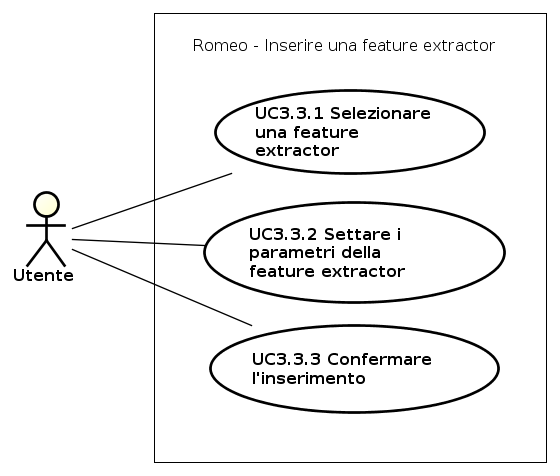
\includegraphics[scale=0.6]{./img/Use_Case/UC3_3}
\caption{UC3.3 - Inserire una feature extractor}
\end{center}
\end{figure}
\begin{itemize}
\item \textbf{Attori:} Utente;
\item \textbf{Scopo e descrizione:} l'utente associa al Protocol\glossario{} che sta creando, una feature extractor\glossario{} tra quelle presenti nel sistema;
\item \textbf{Precondizione:} l'utente ha scelto di inserire una feature extractor\glossario{} nel \protocol{}. Il sistema propone le feature extractors\glossario{} compatibili con il tipo di dato su cui il \protocol{} opererà;
\item \textbf{Flusso principale degli eventi:}
\begin{enumerate}
\item l'utente seleziona la feature extractor\glossario{} tra quelle proposte dal sistema [UC3.3.1];
\item l'utente imposta i parametri della feature extractor\glossario{} che ha scelto di inserire [UC3.3.2];
\item l'utente conferma l'inserimento della feature extractor\glossario{} nel \protocol{} [UC3.3.3].
\end{enumerate}
\item \textbf{Postcondizione:} il sistema aggiorna il Protocol\glossario{} con la feature extractor\glossario{} scelta dall'utente.
\end{itemize}

\subsection{Caso d'uso UC3.3.1: Selezionare una feature extractor}
\begin{itemize}
\item \textbf{Attori:} Utente;
\item \textbf{Scopo e descrizione:} l'utente seleziona una feature extractor\glossario{} tra quelle proposte dal sistema;
\item \textbf{Precondizione:} il sistema visualizza le feature extractor\glossario{} compatibili con il tipo di dato su cui il \protocol{} opererà;
\item \textbf{Flusso principale degli eventi:}
\begin{enumerate}
\item l'utente seleziona la feature extractor\glossario{} tra quelle proposte dal sistema.
\end{enumerate}
\item \textbf{Postcondizione:} il sistema memorizza la feature extractor\glossario{} scelta dall'utente.
\end{itemize}

\subsection{Caso d'uso UC3.3.2: Settare i parametri della feature extractor}
\begin{itemize}
\item \textbf{Attori:} Utente;
\item \textbf{Scopo e descrizione:} l'utente imposta i parametri che utilizzerà la feature extractor\glossario{} per operare;
\item \textbf{Precondizione:} il sistema visualizza i parametri di default definiti per la specifica feature extractor\glossario{}. L'utente ha deciso di non utilizzarli e vuole impostarli manualmente;
\item \textbf{Flusso principale degli eventi:}
\begin{enumerate}
\item l'utente imposta i vari parametri della feature extractor\glossario{}.
\end{enumerate}
\item \textbf{Postcondizione:} il sistema memorizza i parametri della feature extractor\glossario{} decisi dall'utente.
\end{itemize}

\subsection{Caso d'uso UC3.3.3: Confermare l'inserimento}
\begin{itemize}
\item \textbf{Attori:} Utente;
\item \textbf{Scopo e descrizione:} l'utente conferma l'inserimento della feature extractor\glossario{} scelta in precedenza;
\item \textbf{Precondizione:} il sistema ha memorizzato le precedenti scelte dell'utente e permette a quest'ultimo di confermare la propria scelta;
\item \textbf{Flusso principale degli eventi:}
\begin{enumerate}
\item l'utente conferma l'inserimento della feature extractor\glossario{}.
\end{enumerate}
\item \textbf{Postcondizione:} il sistema memorizza l'associazione tra la feature extractor\glossario{} scelta ed impostata dall'utente e il \protocol{}.
\end{itemize}

\subsection{Caso d'uso UC3.4: Inserire un algoritmo di clustering}
\begin{figure}[!h]
\begin{center}
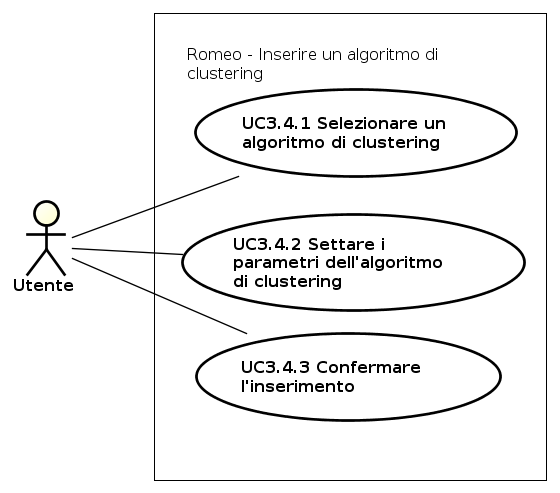
\includegraphics[scale=0.6]{./img/Use_Case/UC3_4}
\caption{UC3.4 - Inserire un algoritmo di clustering}
\end{center}
\end{figure}
\begin{itemize}
\item \textbf{Attori:} Utente;
\item \textbf{Scopo e descrizione:} l'utente associa al \protocol{} che sta creando, un algoritmo di clustering\glossario{} tra quelli proposti dal sistema;
\item \textbf{Precondizione:} l'utente ha deciso di inserire un algoritmo di clustering\glossario{} nel \protocol{}. Il sistema propone gli algoritmi di clustering\glossario{} compatibili con il tipo di dato su cui il \protocol{} opererà;
\item \textbf{Flusso principale degli eventi:}
\begin{enumerate}
\item l'utente seleziona l'algoritmo di clustering\glossario{} tra quelli proposti dal sistema [UC3.4.1];
\item l'utente imposta i parametri dell'algoritmo di clustering\glossario{} che ha scelto di inserire [UC3.4.2];
\item l'utente conferma l'inserimento dell'algoritmo di clustering\glossario{} nel \protocol{} [UC3.4.3].
\end{enumerate}
\item \textbf{Postcondizione:} il sistema aggiorna il Protocol\glossario{} con l'algoritmo di clustering\glossario{} scelto dall'utente.
\end{itemize}

\subsection{Caso d'uso UC3.4.1: Selezionare un algoritmo di clustering}
\begin{itemize}
\item \textbf{Attori:} Utente;
\item \textbf{Scopo e descrizione:} l'utente seleziona un algoritmo di clustering\glossario{} tra quelli proposti dal sistema;
\item \textbf{Precondizione:} il sistema visualizza gli algoritmo di clustering\glossario{} compatibili con il tipo di dato su cui il \protocol{} opererà;
\item \textbf{Flusso principale degli eventi:}
\begin{enumerate}
\item l'utente seleziona l'algoritmo di clustering\glossario{} tra quelli proposti dal sistema.
\end{enumerate}
\item \textbf{Postcondizione:} il sistema memorizza l'algoritmo di clustering\glossario{} scelto dall'utente.
\end{itemize}

\subsection{Caso d'uso UC3.4.2: Settare i parametri dell'algoritmo di clustering}
\begin{itemize}
\item \textbf{Attori:} Utente;
\item \textbf{Scopo e descrizione:} l'utente imposta i parametri che utilizzerà l'algoritmo di clustering\glossario{} per operare;
\item \textbf{Precondizione:} il sistema visualizza i parametri di default definiti per lo specifico algoritmo di clustering\glossario{}. L'utente ha deciso di non utilizzarli e vuole impostarli manualmente;
\item \textbf{Flusso principale degli eventi:}
\begin{enumerate}
\item l'utente imposta i vari parametri dell'algoritmo di clustering\glossario{}.
\end{enumerate}
\item \textbf{Postcondizione:} il sistema memorizza i parametri dell'algoritmo di clustering\glossario{} decisi dall'utente.
\end{itemize}

\subsection{Caso d'uso UC3.4.3: Confermare l'inserimento}
\begin{itemize}
\item \textbf{Attori:} Utente;
\item \textbf{Scopo e descrizione:} l'utente conferma l'inserimento dell'algoritmo di clustering\glossario{} scelto in precedenza;
\item \textbf{Precondizione:} il sistema ha memorizzato le precedenti scelte dell'utente e permette a quest'ultimo di confermare la propria scelta;
\item \textbf{Flusso principale degli eventi:}
\begin{enumerate}
\item l'utente conferma l'inserimento dell'algoritmo di clustering\glossario{}.
\end{enumerate}
\item \textbf{Postcondizione:} il sistema memorizza l'associazione tra l'algoritmo di clustering\glossario{} scelto ed impostato dall'utente e il \protocol{}.
\end{itemize}

\subsection{Caso d'uso UC3.5: Inserire una descrizione}
\begin{itemize}
\item \textbf{Attori:} Utente;
\item \textbf{Scopo e descrizione:} l'utente inserisce una descrizione riguardante il Protocol\glossario{} che sta creando, in modo da facilitare  la comprensione del suo risultato anche a chi non ha creato tale Protocol\glossario{};
\item \textbf{Precondizione:} il sistema mostra la schermata di creazione di un Protocol\glossario{};
\item \textbf{Flusso principale degli eventi:}
\begin{enumerate}
\item L'utente inserisce una descrizione riguardo al Protocol\glossario{} che sta creando.
\end{enumerate}
\item \textbf{Postcondizione:} Il sistema ha memorizzato la descrizione inserita dall'utente e l'ha associata al Protocol\glossario{} in creazione.
\end{itemize}


\subsection{Caso d'uso UC3.6: Salvare il Protocol}
\begin{itemize}
\item \textbf{Attori:} Utente;
\item \textbf{Scopo e descrizione:} l'utente salva il Protocol\glossario{} che ha appena creato;
\item \textbf{Precondizione:} il sistema mostra la schermata di creazione di un Protocol\glossario{};
\item \textbf{Flusso principale degli eventi:}
\begin{enumerate}
\item l'utente salva il Protocol\glossario{}.
\end{enumerate}
\item \textbf{Postcondizione:} il sistema ha salvato il Protocol\glossario{}.
\end{itemize}


%server oer sistemare l'immagine
\subsection{Caso d'uso UC4: Creazione Dataset}
\begin{figure}[!h]
\begin{center}
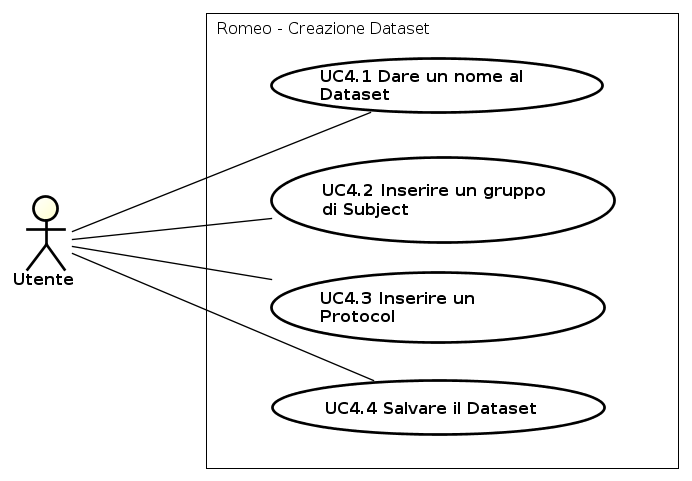
\includegraphics[scale=0.6]{./img/Use_Case/UC4}
\caption{UC4 - Creazione Dataset}
\end{center}
\end{figure}
\begin{itemize}
\item \textbf{Attori:} Utente;
\item \textbf{Scopo e descrizione:} l'utente sta creando un Dataset\glossario{}, quindi in primo luogo, deve assegnargli un nome. Successivamente deve associargli un gruppo di Subject\glossario{} e uno o più Protocol\glossario{} che verranno applicati ai gruppi di Subject\glossario{}. Infine l'utente deve salvare il Dataset\glossario{} appena creato;
\item \textbf{Precondizione:} Nel sistema ci devono essere almeno un gruppo di Subject\glossario{} e un Protocol\glossario{} e l'utente deve aver scelto di creare un Dataset\glossario{};
\item \textbf{Flusso principale degli eventi:} 
\begin{enumerate}
\item l'utente dà un nome al Dataset\glossario{} [UC4.1];
\item l'utente inserisce un gruppo di Subject\glossario{} già esistente [UC4.2];
\item l'utente inserisce un Protocol\glossario{} già esistente [UC4.3];
\item l'utente salva il Dataset\glossario{} [UC4.4].
\end{enumerate}
\item \textbf{Scenario alternativo:} l'utente inserisce un nome già associato ad un altro Dataset\glossario{}; il sistema segnala l'incongruenza e chiede di inserire un nome diverso;
\item \textbf{Postcondizione:} l'utente ha creato un Dataset\glossario{} che è pronto per essere analizzato.
\end{itemize}

\subsection{Caso d'uso UC4.1: Dare un nome al Dataset}
\begin{itemize}
\item \textbf{Attori:} Utente;
\item \textbf{Scopo e descrizione:} l'utente deve dare un nome al Dataset\glossario{} che sta creando, per poterlo identificare successivamente;
\item \textbf{Precondizione:} il sistema è in attesa che l'utente inserisca il nome del Dataset\glossario{};
\item \textbf{Flusso principale degli eventi:}
\begin{enumerate}
\item l'utente dà un nome al Dataset\glossario{}.
\end{enumerate}
\item \textbf{Postcondizione:} il sistema associa al Dataset\glossario{} in creazione, il nome inserito dall'utente.
\end{itemize}

\subsection{Caso d'uso UC4.2: Inserire un gruppo di Subject}
\begin{itemize}
\item \textbf{Attori:} Utente;
\item \textbf{Scopo e descrizione:} l'utente inserisce un gruppo di Subject\glossario{} nel Dataset\glossario{} che sta costruendo;
\item \textbf{Precondizione:} il sistema mostra la schermata di creazione del Dataset\glossario{};
\item \textbf{Flusso principale degli eventi:}
\begin{enumerate}
\item l'utente inserisce un gruppo di Subject\glossario{} nel Dataset\glossario{}.
\end{enumerate}
\item \textbf{Postcondizione:} il sistema aggiunge al Dataset\glossario{} il gruppo di Subject\glossario{} scelto dall'utente.
\end{itemize}

\subsection{Caso d'uso UC4.3: Inserire un Protocol}
\begin{itemize}
\item \textbf{Attori:} Utente;
\item \textbf{Scopo e descrizione:} l'utente inserisce un Protocol\glossario{} nel Dataset\glossario{} che sta costruendo;
\item \textbf{Precondizione:} il sistema mostra la schermata di creazione del Dataset\glossario{};
\item \textbf{Flusso principale degli eventi:}
\begin{enumerate}
\item l'utente inserisce un Protocol\glossario{} nel Dataset\glossario{}.
\end{enumerate}
\item \textbf{Postcondizione:} il sistema ha aggiunto al Dataset\glossario{} il Protocol\glossario{} selezionato dall'utente.
\end{itemize}

\subsection{Caso d'uso UC4.4: Salvare il Dataset}
\begin{itemize}
\item \textbf{Attori:} Utente;
\item \textbf{Scopo e descrizione:} l'utente salva il Dataset\glossario{} che ha appena creato;
\item \textbf{Precondizione:} il sistema mostra la schermata di creazione di un Dataset\glossario{}; l'utente deve aver inserito almeno un gruppo di Subject\glossario{} e almeno un Protocol\glossario{} nel Dataset\glossario{};
\item \textbf{Flusso principale degli eventi:}
\begin{enumerate}
\item l'utente salva il Dataset\glossario{}.
\end{enumerate}
\item \textbf{Postcondizione:} il sistema ha salvato il Dataset\glossario{}.
\end{itemize}

\subsection{Caso d'uso UC5: Gestione gruppi di Subject}
\begin{figure}[!h]
\begin{center}
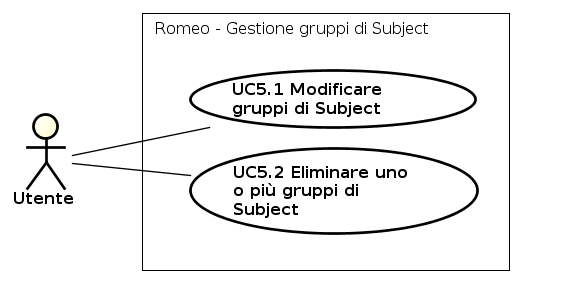
\includegraphics[scale=0.6]{./img/Use_Case/UC5}
\caption{UC5 - Gestione gruppi di Subject}
\end{center}
\end{figure}
\begin{itemize}
\item \textbf{Attori:} Utente;
\item \textbf{Scopo e descrizione:} l'utente vuole compiere delle operazioni sui gruppi di Subject\glossario{} già esistenti;
\item \textbf{Precondizione:} Nel sistema deve essere presente almeno un gruppo di Subject\glossario{} e l'utente deve aver scelto di gestire i gruppi di Subject\glossario{};
\item \textbf{Flusso principale degli eventi:}
\begin{enumerate}
\item l'utente modifica dei gruppi di Subject\glossario{} [UC5.1];
\item l'utente elimina dei gruppi di Subject\glossario{} [UC5.2].
\end{enumerate}
\item \textbf{Postcondizione:} il sistema ha salvato le modifiche o le eliminazioni effettuate dall'utente.
\end{itemize}

\pagebreak

\subsection{Caso d'uso UC5.1: Modificare gruppi di Subject}
\begin{figure}[!h]
\begin{center}
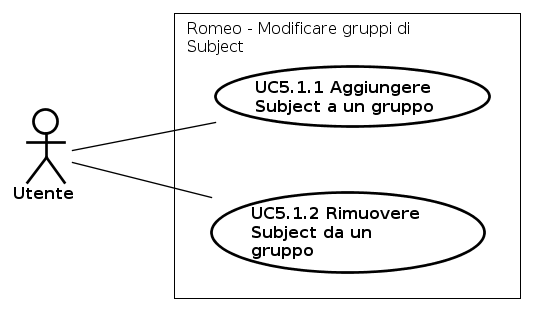
\includegraphics[scale=0.6]{./img/Use_Case/UC5_1}
\caption{UC5.1 - Modificare gruppi di Subject}
\end{center}
\end{figure}
\begin{itemize}
\item \textbf{Attori:} Utente;
\item \textbf{Scopo e descrizione:} l'utente può aggiungere o rimuovere dei Subject\glossario{} appartenenti ad un gruppo già esistente;
\item \textbf{Precondizione:} il sistema è in attesa che l'utente scelga l'operazione che desidera effettuare;
\item \textbf{Flusso principale degli eventi:}
\begin{enumerate}
\item l'utente può aggiungere dei Subject\glossario{} ad un gruppo già esistente UC[5.1.1];
\item l'utente può rimuovere dei Subject\glossario{} da un gruppo già esistente [UC5.1.2].
\end{enumerate}
\item \textbf{Postcondizione:} il sistema ha aggiunto o rimosso i Subject\glossario{} indicati dall'utente.
\end{itemize}

\subsection{Caso d'uso UC5.1.1: Aggiungere Subject ad un gruppo}

\begin{figure}[!h]
\begin{center}
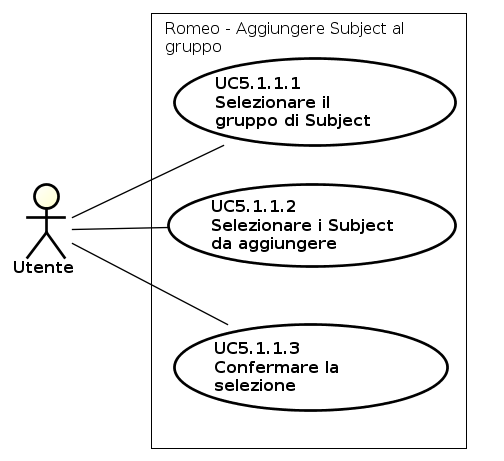
\includegraphics[scale=0.6]{./img/Use_Case/UC5_1_1}
\caption{UC5.1.1 - Aggiungere Subject ad un gruppo}
\end{center}
\end{figure}
\begin{itemize}
\item \textbf{Attori:} Utente;
\item \textbf{Scopo e descrizione:} l'utente aggiunge dei Subject\glossario{} ad un gruppo già esistente;
\item \textbf{Precondizione:} il sistema mostra i gruppi di Subject\glossario{} memorizzati e l'utente ha scelto di aggiungere dei Subject\glossario{} all'interno di un gruppo;
\item \textbf{Flusso principale degli eventi:}
\begin{enumerate}
\item l'utente seleziona un gruppo di Subject\glossario{} [UC5.1.1.1];
\item l'utente seleziona i Subject\glossario{} da aggiungere [UC5.1.1.2];
\item l'utente conferma di voler aggiungere i Subject\glossario{} selezionati [UC5.1.1.3].
\end{enumerate}
\item \textbf{Postcondizione:} il gruppo di Subject\glossario{} è stato aggiornato aggiungendo i Subject\glossario{} selezionati dall'utente.
\end{itemize}


\subsection{Caso d'uso UC5.1.1.1: Selezionare un gruppo di Subject}
\begin{itemize}
\item \textbf{Attori:} Utente;
\item \textbf{Scopo e descrizione:} l'utente seleziona il gruppo di Subject\glossario{} a cui vuole aggiungere dei Subject\glossario{};
\item \textbf{Precondizione:} il sistema mostra la schermata di aggiunta Subject\glossario{} ad un gruppo;
\item \textbf{Flusso principale degli eventi:}
\begin{enumerate}
\item l'utente seleziona un gruppo di Subject\glossario{}.
\end{enumerate}
\item \textbf{Postcondizione:} il sistema mostra all'utente i Subject\glossario{} compatibili con il gruppo, in base al tipo di formato delle immagini.
\end{itemize}

\subsection{Caso d'uso UC5.1.1.2: Selezionare i Subject da aggiungere}
\begin{itemize}
\item \textbf{Attori:} Utente;
\item \textbf{Scopo e descrizione:} l'utente seleziona da un elenco i Subject\glossario{} che vuole aggiungere;
\item \textbf{Precondizione:} il sistema mostra all'utente una lista di Subject\glossario{} ed è in attesa che l'utente li scelga;
\item \textbf{Flusso principale degli eventi:}
\begin{enumerate}
\item l'utente seleziona i Subject\glossario{} da aggiungere.
\end{enumerate}
\item \textbf{Postcondizione:} il sistema sa quali Subject\glossario{} l'utente vuole aggiungere al gruppo.
\end{itemize}

\subsection{Caso d'uso UC5.1.1.3: Confermare la selezione}
\begin{itemize}
\item \textbf{Attori:} Utente;
\item \textbf{Scopo e descrizione:} l'utente conferma di voler inserire nel gruppo i Subject\glossario{} precedentemente selezionati;
\item \textbf{Precondizione:} il sistema è in attesa della conferma da  parte dell'utente;
\item \textbf{Flusso principale degli eventi:}
\begin{enumerate}
\item l'utente conferma di voler inserire i Subject\glossario{} precedentemente selezionati.
\end{enumerate}
\item \textbf{Postcondizione:} il sistema ha aggiornato il gruppo, aggiungendo i Subject\glossario{} selezionati dall'utente.
\end{itemize}


\subsection{Caso d'uso UC5.1.2: Rimuovere Subject da un gruppo}
\begin{figure}[!h]
\begin{center}
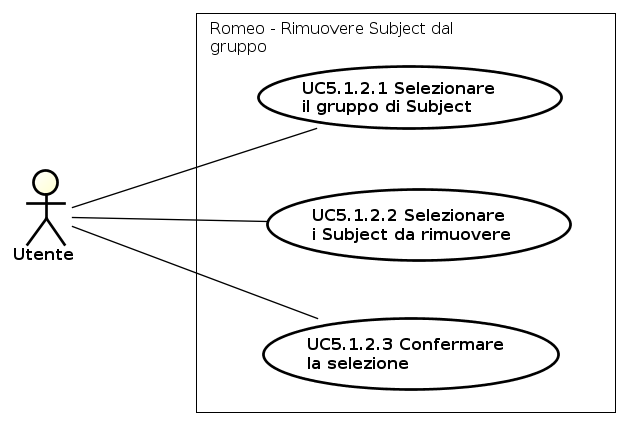
\includegraphics[scale=0.6]{./img/Use_Case/UC5_1_2}
\caption{UC5.1.2 - Rimuovere Subject da un gruppo}
\end{center}
\end{figure}
\begin{itemize}
\item \textbf{Attori:} Utente;
\item \textbf{Scopo e descrizione:} l'utente rimuove dei Subject\glossario{} da un gruppo esistente;
\item \textbf{Precondizione:} il sistema mostra i gruppi di Subject\glossario{} memorizzati in esso e l'utente ha deciso di rimuovere uno o più Subject\glossario{} da un gruppo;
\item \textbf{Flusso principale degli eventi:}
\begin{enumerate}
\item l'utente seleziona un gruppo di Subject\glossario{} [UC5.1.2.1];
\item l'utente seleziona i Subject\glossario{} da rimuovere [UC5.1.2.2];
\item l'utente conferma di voler rimuovere i Subject\glossario{} selezionati [UC5.1.2.3].
\end{enumerate}
\item \textbf{Postcondizione:} il gruppo di Subject\glossario{} è stato aggiornato rimuovendo i Subject\glossario{} selezionati dall'utente.
\end{itemize}


\subsection{Caso d'uso UC5.1.2.1: Selezionare un gruppo di Subject}
\begin{itemize}
\item \textbf{Attori:} Utente;
\item \textbf{Scopo e descrizione:} l'utente seleziona un gruppo da cui vuole rimuovere dei Subject\glossario{};
\item \textbf{Precondizione:} il sistema mostra la schermata di rimozione Subject\glossario{} da un gruppo;
\item \textbf{Flusso principale degli eventi:}
\begin{enumerate}
\item l'utente seleziona un gruppo di Subject\glossario{} già esistente.
\end{enumerate}
\item \textbf{Postcondizione:} il sistema mostra all'utente i Subject\glossario{} contenuti nel gruppo selezionato.
\end{itemize}

\subsection{Caso d'uso UC5.1.2.2: Selezionare i Subject da rimuovere}
\begin{itemize}
\item \textbf{Attori:} Utente;
\item \textbf{Scopo e descrizione:} l'utente seleziona da un elenco i Subject\glossario{} che vuole rimuovere;
\item \textbf{Precondizione:} il sistema mostra all'utente una lista di Subject\glossario{};
\item \textbf{Flusso principale degli eventi:}
\begin{enumerate}
\item l'utente seleziona i Subject\glossario{} che intende rimuovere dal gruppo.
\end{enumerate}
\item \textbf{Postcondizione:} il sistema sa quali Subject\glossario{} l'utente vuole rimuovere dal gruppo.
\end{itemize}

\subsection{Caso d'uso UC5.1.2.3: Confermare la selezione}
\begin{itemize}
\item \textbf{Attori:} Utente;
\item \textbf{Scopo e descrizione:} l'utente conferma di voler rimuovere dal gruppo i Subject\glossario{} precedentemente selezionati;
\item \textbf{Precondizione:} il sistema è in attesa della conferma da parte dell'utente;
\item \textbf{Flusso principale degli eventi:}
\begin{enumerate}
\item l'utente conferma di voler eliminare dal gruppo i Subject\glossario{} precedentemente selezionati.
\end{enumerate}
\item \textbf{Postcondizione:} il sistema ha aggiornato il gruppo, rimuovendo i Subject\glossario{} selezionati dall'utente.
\end{itemize}


\subsection{Caso d'uso UC5.2: Eliminare gruppi di Subject}
\begin{figure}[!h]
\begin{center}
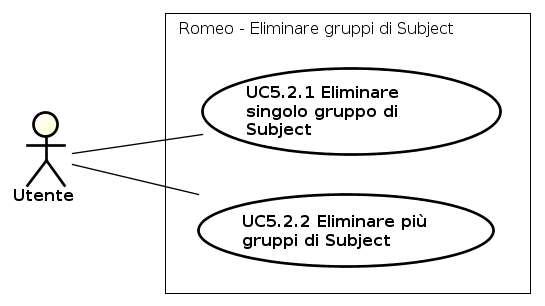
\includegraphics[scale=0.6]{./img/Use_Case/UC5_2}
\caption{UC5.2 - Eliminare gruppi di Subject}
\end{center}
\end{figure}
\begin{itemize}
\item \textbf{Attori:} Utente;
\item \textbf{Scopo e descrizione:} l'utente desidera eliminare gruppi di Subject\glossario{};
\item \textbf{Precondizione:} il sistema mostra la schermata di eliminazione gruppi di Subject\glossario{} e l'utente ha deciso di eliminare un gruppo di Subject\glossario{};
\item \textbf{Flusso principale degli eventi:}
\begin{enumerate}
\item l'utente desidera eliminare un solo gruppo di Subject\glossario{} [UC5.2.1];
\item l'utente desidera eliminare più di un gruppo di Subject\glossario{} [UC5.2.2].
\end{enumerate}
\item \textbf{Postcondizione:} il sistema ha eliminato i gruppi di Subject\glossario{} scelti dall'utente.
\end{itemize}


\subsection{Caso d'uso UC5.2.1: Eliminare un singolo gruppo di Subject}
\begin{figure}[!h]
\begin{center}
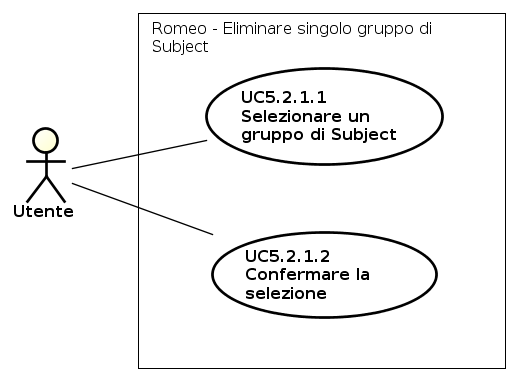
\includegraphics[scale=0.6]{./img/Use_Case/UC5_2_1}
\caption{UC5.2.1 - Eliminare un singolo gruppo di Subject}
\end{center}
\end{figure}
\begin{itemize}
\item \textbf{Attori:} Utente;
\item \textbf{Scopo e descrizione:} l'utente desidera eliminare un singolo gruppo di Subject\glossario{} tra quelli presenti nel sistema, dunque dovrà selezionare il gruppo che desidera eliminare e in seguito confermare tale selezione;
\item \textbf{Precondizione:} il sistema mostra la schermata di eliminazione gruppi di Subject\glossario{}, l'utente deve aver scelto di eliminare un singolo gruppo di \subject{};
\item \textbf{Flusso principale degli eventi:}
\begin{enumerate}
\item l'utente seleziona un gruppo di Subject\glossario{} [UC5.2.1.1];
\item l'utente conferma di voler eliminare il gruppo di Subject\glossario{} selezionato in precedenza [UC5.2.1.2].
\end{enumerate}
\item \textbf{Postcondizione:} il sistema ha eliminato il gruppo di Subject\glossario{} indicato dall'utente.
\end{itemize}

\subsection{Caso d'uso UC5.2.1.1: Selezionare un gruppo di Subject}
\begin{itemize}
\item \textbf{Attori:} Utente;
\item \textbf{Scopo e descrizione:} l'utente seleziona tra i gruppi proposti dal sistema, quello che desidera eliminare;
\item \textbf{Precondizione:} il sistema mostra la lista dei gruppi di Subject\glossario{} presenti in esso;
\item \textbf{Flusso principale degli eventi:}
\begin{enumerate}
\item l'utente seleziona un gruppo di Subject\glossario{}.
\end{enumerate}
\item \textbf{Postcondizione:} il sistema conosce il gruppo di Subject\glossario{} che l'utente desidera eliminare.
\end{itemize}

\subsection{Caso d'uso UC5.2.1.2: Confermare la selezione}
\begin{itemize}
\item \textbf{Attori:} Utente;
\item \textbf{Scopo e descrizione:} l'utente conferma di voler eliminare il gruppo di Subject\glossario{} che ha selezionato in precedenza;
\item \textbf{Precondizione:} il sistema ha un gruppo di Subject\glossario{} selezionato ed è in attesa della conferma da parte dell'utente;
\item \textbf{Flusso principale degli eventi:}
\begin{enumerate}
\item l'utente conferma di voler eliminare il gruppo di Subject\glossario{} precedentemente selezionato.
\end{enumerate}
\item \textbf{Postcondizione:} il sistema ha eliminato il gruppo di Subject\glossario{} selezionato in precedenza dall'utente.
\end{itemize}


\subsection{Caso d'uso UC5.2.2: Eliminare più gruppi di Subject}
\begin{figure}[!h]
\begin{center}
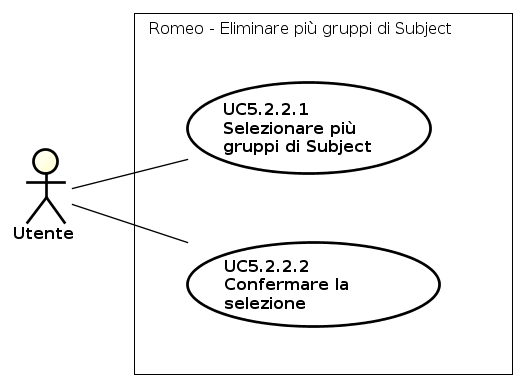
\includegraphics[scale=0.6]{./img/Use_Case/UC5_2_2}
\caption{UC5.2.2 - Eliminare più gruppi di Subject}
\end{center}
\end{figure}
\begin{itemize}
\item \textbf{Attori:} Utente;
\item \textbf{Scopo e descrizione:} l'utente desidera eliminare più di un gruppo di Subject\glossario{}, seleziona quindi quelli che vuole eliminare e conferma al sistema la sua selezione; 
\item \textbf{Precondizione:} il sistema ha dei gruppi di Subject\glossario{} all'interno di esso, l'utente ha scelto di eliminare più di un gruppo di Subject\glossario{};
\item \textbf{Flusso principale degli eventi:}
\begin{enumerate}
\item l'utente seleziona più di un gruppo di Subject\glossario{} tra quelli proposti dal sistema [UC5.2.2.1];
\item l'utente conferma di voler eliminare i gruppi di Subject\glossario{} precedentemente selezionati [UC5.2.2.2].
\end{enumerate}
\item \textbf{Postcondizione:} il sistema ha eliminato i gruppi di Subject\glossario{} selezionati in precedenza dall'utente.
\end{itemize}

\subsection{Caso d'uso UC5.2.2.1: Selezionare più gruppi di Subject}
\begin{itemize}
\item \textbf{Attori:} Utente;
\item \textbf{Scopo e descrizione:} l'utente seleziona almeno due gruppi di Subject\glossario{} da eliminare successivamente;
\item \textbf{Precondizione:} l'utente mostra la lista dei gruppi di Subject\glossario{} esistenti;
\item \textbf{Flusso principale degli eventi:}
\begin{enumerate}
\item l'utente seleziona più gruppi di Subject\glossario{}.
\end{enumerate}
\item \textbf{Postcondizione:} il sistema conosce i gruppi di Subject\glossario{} che l'utente desidera eliminare.
\end{itemize} 

\subsection{Caso d'uso UC5.2.2.2: Confermare la selezione}
\begin{itemize}
\item \textbf{Attori:} Utente;
\item \textbf{Scopo e descrizione:} l'utente conferma d voler eliminare i gruppi di Subject\glossario{} selezionati in precedenza;
\item \textbf{Precondizione:} l'utente deve aver precedentemente selezionato dei gruppi d Subject\glossario{} da eliminare;
\item \textbf{Flusso principale degli eventi:}
\begin{enumerate}
\item l'utente conferma di voler eliminare i gruppi di Subject\glossario{} selezionati in precedenza.
\end{enumerate}
\item \textbf{Postcondizione:} il sistema ha eliminato i gruppi di Subject\glossario{} selezionati in precedenza dall'utente.
\end{itemize}

\subsection{Caso d'uso UC6: Eliminazione Protocol}
\begin{figure}[!h]
\begin{center}
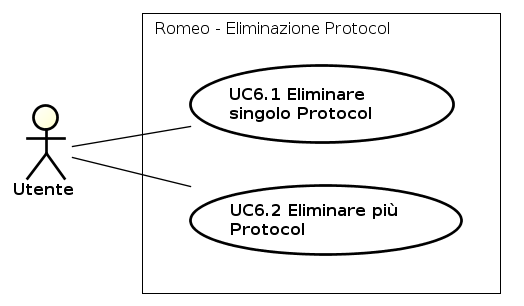
\includegraphics[scale=0.6]{./img/Use_Case/UC6}
\caption{UC6 - Eliminazione Protocol}
\end{center}
\end{figure}
\begin{itemize}
\item \textbf{Attori:} Utente;
\item \textbf{Scopo e descrizione:}l'utente deve eliminare dei Protocol\glossario{} e può scegliere se eliminarli singolarmente o eliminarne un gruppo;
\item \textbf{Precondizione:} il sistema mostra la schermata di eliminazione Protocol\glossario{}, l'utente deve aver scelto di eliminare Protocol\glossario{};
\item \textbf{Flusso principale delle azioni:}
\begin{enumerate}
\item l'utente desidera eliminare un singolo Protocol\glossario{} [UC6.1];
\item l'utente desidera eliminare più di un Protocol\glossario{} [UC6.2].
\end{enumerate}
\item \textbf{Postcondizione:} il sistema ha eliminato i Protocol\glossario{} indicati dall'utente.
\end{itemize}


\subsection{Caso d'uso UC6.1: Eliminare un Protocol}
\begin{figure}[!h]
\begin{center}
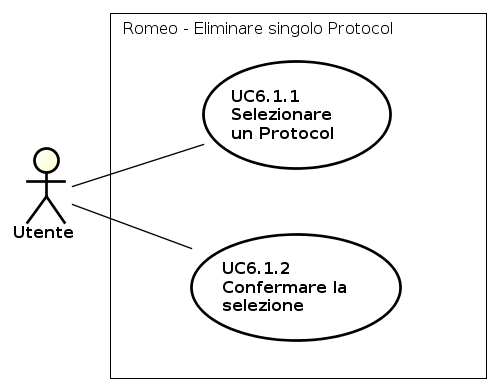
\includegraphics[scale=0.6]{./img/Use_Case/UC6_1}
\caption{UC6.1 - Eliminare un singolo Protocol}
\end{center}
\end{figure}
\begin{itemize}
\item \textbf{Attori:} Utente;
\item \textbf{Scopo e descrizione:} l'utente desidera eliminare un singolo Protocol\glossario{}, egli dovrà quindi selezionare un Protocol\glossario{} {} e confermare di volerlo eliminare dal sistema;
\item \textbf{Precondizione}: il sistema mostra all'utente la lista di Protocol\glossario{} presenti nel sistema, l'utente ha scelto di eliminare un unico Protocol\glossario{};
\item \textbf{Flusso principale delle azioni:}
\begin{enumerate}
\item l'utente seleziona un Protocol\glossario{} [UC6.1.1];
\item l'utente conferma di voler eliminare il \protocol{} precedentemente indicato [UC6.1.2].
\end{enumerate}
\item \textbf{Postcondizione:} il sistema ha eliminato il Protocol\glossario{} indicato dall'utente.
\end{itemize}

\subsection{Caso d'uso UC6.1.1: Selezionare un singolo Protocol}
\begin{itemize}
\item \textbf{Attori:} Utente;
\item \textbf{Scopo e descrizione:} l'utente seleziona un singolo Protocol\glossario{} da una lista proposta dal sistema;
\item \textbf{Precondizione:} il sistema mostra la lista dei Protocol\glossario{} presenti nel sistema;
\item \textbf{Flusso principale degli eventi:}
\begin{enumerate}
\item l'utente seleziona un Protocol\glossario{}.
\end{enumerate}
\item \textbf{Postcondizione: } il sistema conosce il Protocol\glossario{} che l'utente desidera eliminare.
\end{itemize}

\subsection{Caso d'uso UC6.1.2: Confermare la selezione}
\begin{itemize}
\item \textbf{Attori:} Utente;
\item \textbf{Scopo e descrizione:} l'utente conferma di voler eliminare il Protocol\glossario{} precedentemente selezionato;
\item \textbf{Precondizione:} l'utente deve aver precedentemente selezionato un Protocol
\item \textbf{Flusso principale degli eventi:}
\begin{enumerate}
\item l'utente conferma di voler eliminare il Protocol\glossario{}.
\end{enumerate}
\item \textbf{Postcondizione:} il sistema ha eliminato il Protocol\glossario{} scelto dall'utente.
\end{itemize}

\subsection{Caso d'uso UC6.2: Eliminare più Protocol}
\begin{figure}[!h]
\begin{center}
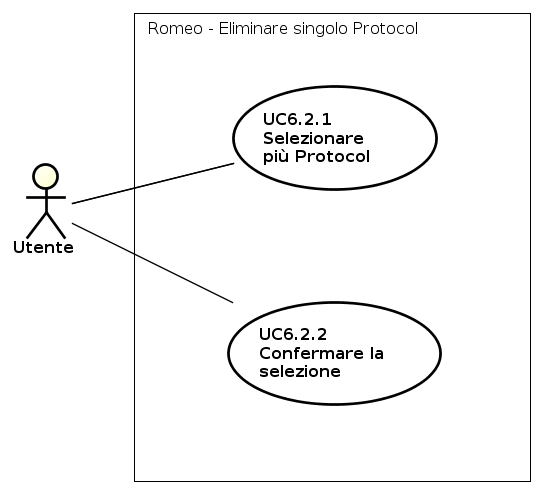
\includegraphics[scale=0.6]{./img/Use_Case/UC6_2}
\caption{UC6.2 - Eliminare più Protocol}
\end{center}
\end{figure}
\begin{itemize}
\item \textbf{Attori:} Utente;
\item \textbf{Scopo e descrizione:} l'utente desidera eliminare almeno due Protocol\glossario{}, egli dovrà quindi selezionare i Protocol\glossario{} {} e confermare di volerli eliminare dal sistema;
\item \textbf{Precondizione:} il sistema mostra la schermata di eliminazione Protocol\glossario{}, l'utente deve aver scelto di eliminare Protocol\glossario{};
\item \textbf{Flusso principale degli eventi: }
\begin{enumerate}
\item l'utente seleziona almeno due Protocol\glossario{} [UC6.2.1];
\item l'utente conferma di voler eliminare i Protocol\glossario{} selezionati in precedenza [UC6.2.2].
\end{enumerate}
\item \textbf{Postcondizione:} il sistema ha eliminato i Protocol\glossario{} scelti dall'utente.
\end{itemize}


\subsection{Caso d'uso UC6.2.1: Selezionare più Protocol}
\begin{itemize}
\item \textbf{Attori:} Utente;
\item \textbf{Scopo e descrizione:} l'utente seleziona almeno due Protocol\glossario{} da una lista proposta dal sistema;
\item \textbf{Precondizione:} il sistema mostra la lista dei Protocol\glossario{} presenti nel sistema;
\item \textbf{Flusso principale degli eventi:}
\begin{enumerate}
\item l'utente seleziona almeno due Protocol\glossario{}.
\end{enumerate}
\item \textbf{Postcondizione: } il sistema conosce i Protocol\glossario{} che l'utente desidera eliminare.
\end{itemize}


\subsection{Caso d'uso UC6.2.2: Confermare la selezione}
\begin{itemize}
\item \textbf{Attori:} Utente;
\item \textbf{Scopo e descrizione:} l'utente conferma di voler eliminare i Protocol\glossario{} precedentemente selezionati;
\item \textbf{Precondizione:} l'utente deve aver precedentemente selezionato almeno due Protocol
\item \textbf{Flusso principale degli eventi:}
\begin{enumerate}
\item l'utente conferma di voler eliminare i Protocol\glossario{}.
\end{enumerate}
\item \textbf{Postcondizione:} il sistema ha eliminato ii Protocol\glossario{} scelti dall'utente.
\end{itemize}

\pagebreak

\subsection{Caso d'uso UC7: Esecuzione analisi}
\begin{figure}[!h]
\begin{center}
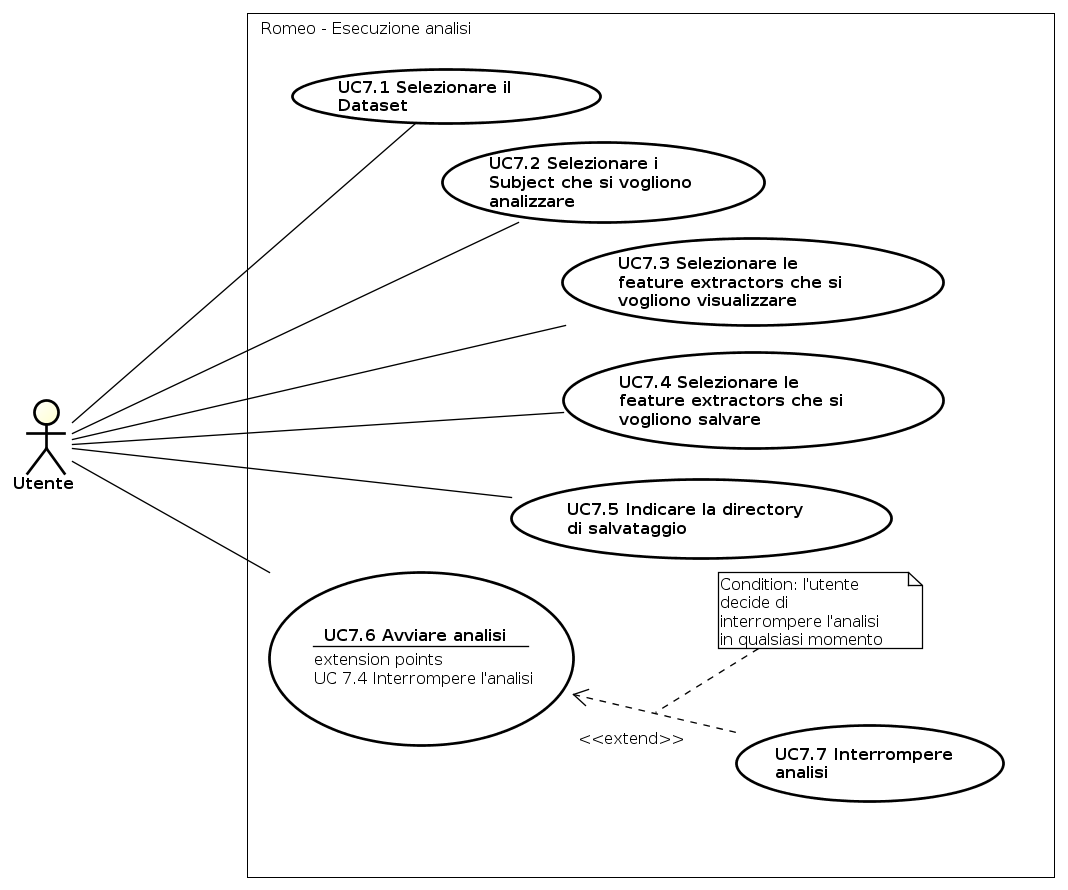
\includegraphics[scale=0.5]{./img/Use_Case/UC7}
\caption{UC7 - Esecuzione analisi}
\end{center}
\end{figure}
\begin{itemize}
\item \textbf{Attori:} Utente;
\item \textbf{Scopo e descrizione:} l'utente vuole effettuare l'analisi di un Dataset\glossario{}. Deve quindi selezionare il Dataset\glossario{} ed eventualmente selezionare i Subject\glossario{} che desidera analizzare. Può inoltre scegliere quali risultati delle feature extractors\glossario{} salvare e di questi, quali visualizzare durante l'analisi. Infine deve indicare la directory in cui salvare i risultati ed avviare l'analisi.
\item \textbf{Precondizione:} Nel sistema deve essere presente almeno un Dataset\glossario{} e l'utente deve aver scelto di effettuare l'analisi;
\item \textbf{Flusso principale degli eventi:}
\begin{enumerate}
	\item l'utente seleziona il Dataset\glossario{} [UC7.1];
	\item l'utente può selezionare i Subject\glossario{} sui quali vuole effettuare l'analisi [UC7.2];
	\item l'utente seleziona le feature extractors\glossario{} di cui vuole salvare il risultato [UC7.3];
	\item l'utente seleziona le feature extractors\glossario{} di cui vuole visualizzare il risultato durante l'analisi [UC7.4];
	\item l'utente indica la directory in cui \project{} deve salvare i risultati [UC7.5];
	\item l'utente avvia l'analisi [UC7.6].
\end{enumerate}
\item \textbf{Estensioni:}
\begin{enumerate}
	\item l'utente può in qualsiasi momento interrompere l'analisi [UC7.7].
\end{enumerate}
\item \textbf{Postcondizione:} L'analisi è terminata e il sistema ha salvato i risultati nella directory indicata nel gruppo di Subject\glossario{}. L'analisi è stata interrotta dall'utente e il sistema ritorna allo stato precedente all'avvio dell'analisi.
\end{itemize}

\subsection{Caso d'uso UC7.1: Selezionare Dataset}
\begin{itemize}
\item \textbf{Attori:} Utente;
\item \textbf{Scopo e descrizione:} l'utente seleziona il Dataset\glossario{} che vuole analizzare;
\item \textbf{Precondizione:} il sistema visualizza i Dataset\glossario{} che si possono analizzare;
\item \textbf{Flusso principale degli eventi:}
\begin{enumerate}
\item l'utente seleziona il Dataset\glossario{} del quale vuole effettuare l'analisi. 
\end{enumerate}
\item \textbf{Postcondizione:} il sistema evidenzia il Dataset\glossario{} selezionato dall'utente e mostra i Subject\glossario{} presenti nel gruppo contenuto nel Dataset\glossario{}.
\end{itemize}

\subsection{Caso d'uso UC7.2: Selezionare i Subject che si vogliono analizzare}
\begin{itemize}
\item \textbf{Attori:} Utente;
\item \textbf{Scopo e descrizione:} l'utente seleziona i Subject\glossario{} di cui vuole effettuare l'analisi;
\item \textbf{Precondizione:} il sistema visualizza i Subject\glossario{} contenuti nel Dataset\glossario{} precedentemente selezionato;
\item \textbf{Flusso principale degli eventi:}
\begin{enumerate}
\item l'utente seleziona i \subject{} di cui vole effettuare l'analisi.
\end{enumerate}
\item \textbf{Postcondizione:} il sistema sa quali Subject\glossario{} l'utente vuole analizzare.
\end{itemize}

\subsection{Caso d'uso UC7.3: Selezionare le feature extractors che si vogliono visualizzare}
\begin{itemize}
\item \textbf{Attori:} Utente;
\item \textbf{Scopo e descrizione:} l'utente può selezionare le feature extractors\glossario{} di cui desidera visualizzare il risultato durante l'analisi;
\item \textbf{Precondizione:} il sistema visualizza le feature extractors\glossario{} presenti nei Protocol\glossario{} contenuti nel Dataset\glossario{} precedentemente selezionato;
\item \textbf{Flusso principale degli eventi}
\begin{enumerate}
\item l'utente seleziona le feature extractors\glossario{} di cui vuole visualizzare i risultati durante l'analisi.
\end{enumerate}
\item \textbf{Postcondizione:} il sistema sa di quali feature extractors\glossario{} l'utente vuole visualizzare i risultati.
\end{itemize}


\subsection{Caso d'uso UC7.4: Selezionare le feature extractors che si vogliono salvare}
\begin{itemize}
\item \textbf{Attori:} Utente;
\item \textbf{Scopo e descrizione:} l'utente può selezionare le feature extractors\glossario{} di cui desidera salvare il risultato;
\item \textbf{Precondizione:} il sistema visualizza le feature extractors\glossario{} presenti nei Protocol\glossario{} contenuti nel Dataset\glossario{} precedentemente selezionato;
\item \textbf{Flusso principale degli eventi}
\begin{enumerate}
\item l'utente seleziona le feature extractors\glossario{} di cui vuole salvare i risultati.
\end{enumerate}
\item \textbf{Postcondizione:} il sistema sa di quali feature extractors\glossario{} l'utente vuole salvare i risultati.
\end{itemize}

\subsection{Caso d'uso UC7.5: Indicare la directory di salvataggio}
\begin{itemize}
\item \textbf{Attori:} Utente;
\item \textbf{Scopo e descrizione:} l'utente deve specificare la directory in cui verranno salvati i risultati dell'analisi;
\item \textbf{Precondizione:} il sistema mostra la schermata di avvio dell'analisi;
\item \textbf{Flusso principale degli eventi:}
\begin{enumerate}
\item l'utente indica la directory in cui desidera vengano salvati i risultati.
\end{enumerate}
\item \textbf{Postcondizione:} il sistema ha indicato il percorso in cui verranno salvati i risultati delle analisi.
\end{itemize}

\subsection{Caso d'uso UC7.6: Avviare analisi}
\begin{itemize}
\item \textbf{Attori:} Utente;
\item \textbf{Scopo e descrizione:} l'utente avvia l'analisi del Dataset\glossario{} precedentemente selezionato;
\item \textbf{Precondizione:} il sistema ha un Dataset\glossario{}, selezionato precedentemente, sul quale effettuare l'analisi;
\item \textbf{Flusso principale degli eventi:}
\begin{enumerate}
\item l'utente avvia l'analisi.
\end{enumerate}
\item \textbf{Postcondizione:} il sistema ha avviato l'analisi del Dataset\glossario{} precedentemente selezionato.
\end{itemize}

%da sistemare

\subsection{Caso d'uso UC7.7: Interrompere analisi}
\begin{itemize}
\item \textbf{Attori:} Utente;
\item \textbf{Scopo e descrizione:} l'utente può interrompere l'analisi, in qualsiasi momento durante l'esecuzione;
\item \textbf{Precondizione:} l'utente ha precedentemente avviato l'analisi e questa è ancora in corso;
\item \textbf{Flusso principale degli eventi:} 
\begin{enumerate}
\item l'utente interrompe l'analisi.
\end{enumerate}
\item \textbf{Postcondizione:} il sistema ha interrotto l'analisi e mostra la schermata di avvio analisi.
\end{itemize}


\subsection{Caso d'uso UC8: Visualizzazione risultati}
\begin{figure}[!h]
\begin{center}
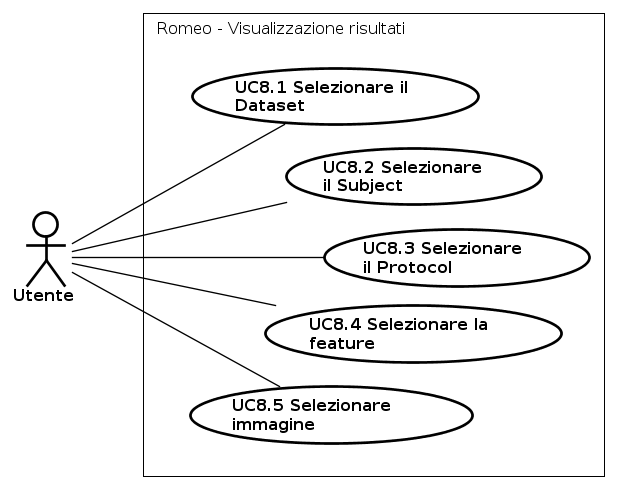
\includegraphics[scale=0.6]{./img/Use_Case/UC8}
\caption{UC8 - Visualizzazione risultati}
\end{center}
\end{figure}
\begin{itemize}
\item \textbf{Attori:} Utente;
\item \textbf{Scopo e descrizione:} l'utente vuole visualizzare i risultati di un'analisi effettuata in precedenza. Egli deve selezionare il Dataset\glossario{} e scegliere il particolare Subject\glossario{} di cui vuole visualizzare il risultato. Successivamente deve selezionare il Protocol\glossario{}, la feature extractor\glossario{} di cui vuole visualizzare il risultato e infine l'immagine corrispondente al risultato;
\item \textbf{Precondizione:} l'utente deve già aver effettuato un'analisi senza aver poi eliminato il gruppo o i gruppi di Subject\glossario{} su cui l'analisi è stata effettuata. Inoltre deve aver deciso di visualizzare i risultati di un'analisi;
\item \textbf{Flusso principale degli eventi:}
\begin{enumerate}
\item l'utente seleziona il Dataset\glossario{} [UC8.1];
\item l'utente seleziona un Subject\glossario{} appartenente ad un gruppo presente all'interno del Dataset\glossario{} [UC8.2];
\item l'utente seleziona il Protocol\glossario{} del quale vuole visualizzare il risultato [UC8.3];
\item l'utente seleziona la feature extractor\glossario{} del quale vuole visualizzare il risultato [UC8.4];
\item l'utente seleziona l'immagine corrispondente alla feature extractor\glossario{} selezionata precedentemente [UC8.5].
\end{enumerate}
\item \textbf{Postcondizione:} l'utente ha visualizzato il risultato relativo alla seleziona precedentemente fatta.
\end{itemize}

\subsection{Caso d'uso UC8.1: Selezionare il Dataset}
\begin{itemize}
\item \textbf{Attori:} Utente;
\item \textbf{Scopo e descrizione:} l'utente seleziona il Dataset\glossario{} dove sono contenuti i risultati che vuole visualizzare;
\item \textbf{Precondizione:} il sistema mostra i Dataset\glossario{} contenuti al suo interno;
\item \textbf{Flusso principale degli eventi:}
\begin{enumerate}
\item l'utente seleziona un Dataset\glossario{} di cui è già stata effettuata l'analisi; 
\end{enumerate}
\item \textbf{Postcondizione:} il sistema visualizza i Subject\glossario{} contenuti nel gruppo associato al Dataset\glossario{} selezionato.
\end{itemize}


\subsection{Caso d'uso UC8.2: Selezionare il Subject}
\begin{itemize}
\item \textbf{Attori:} Utente;
\item \textbf{Scopo e descrizione:} l'utente seleziona il Subject\glossario{} di cui vuole visualizzare i risultati;
\item \textbf{Precondizione:} il sistema visualizza i Subject\glossario{} presenti nel gruppo di Subject\glossario{} contenuto nel Dataset\glossario{};
\item \textbf{Flusso principale degli eventi:}
\begin{enumerate}
\item l'utente seleziona un Subject\glossario{} contenuto nel Dataset\glossario{} precedentemente selezionato.
\end{enumerate}
\item \textbf{Postcondizione:} il sistema evidenzia il Subject\glossario{} selezionato dall'utente.
\end{itemize}

\subsection{Caso d'uso UC8.3: Selezionare il Protocol}
\begin{itemize}
\item \textbf{Attori:} Utente;
\item \textbf{Scopo e descrizione:} l'utente seleziona il Protocol\glossario{} di cui vuole visualizzare i risultati;
\item \textbf{Precondizione:} il sistema visualizza i Protocol\glossario{} presenti nel Dataset\glossario{} precedentemente selezionato;
\item \textbf{Flusso principale degli eventi:}
\begin{enumerate}
\item l'utente seleziona un Protocol\glossario{} contenuto nel Dataset\glossario{} selezionato in precedenza.
\end{enumerate}
\item \textbf{Postcondizione:} il sistema evidenzia il Protocol\glossario{} selezionato dall'utente.
\end{itemize}

\subsection{Caso d'uso UC8.4: Selezionare la feature}
\begin{itemize}
\item \textbf{Attori:} Utente;
\item \textbf{Scopo e descrizione:} l'utente seleziona il feature\glossario{} di cui vuole visualizzare i risultati;
\item \textbf{Precondizione:} il sistema visualizza le feature\glossario{} presenti nel Protocol\glossario{} precedentemente selezionato;
\item \textbf{Flusso principale degli eventi:}
\begin{enumerate}
\item l'utente seleziona una feature\glossario{} contenuta nel Protocol\glossario{} selezionato in precedenza.
\end{enumerate}
\item \textbf{Postcondizione:} il sistema mostra i risultati della feature extractor\glossario{} selezionata dall'utente.
\end{itemize}

\subsection{Caso d'uso UC8.5: Selezionare l'immagine}
\begin{itemize}
\item \textbf{Attori:} Utente;
\item \textbf{Scopo e descrizione:} l'utente seleziona l'immagine relativa alla feature extractor\glossario{} precedentemente selezionata;
\item \textbf{Precondizione:} l'utente ha selezionato precedentemente una feature extractor\glossario{}, il sistema mostra i risultati di tale feature extractor\glossario{};
\item \textbf{Flusso principale degli eventi:}
\begin{enumerate}
\item l'utente seleziona l'immagine.
\end{enumerate}
\item \textbf{Postcondizione:} il sistema mostra il risultato della feature extractor\glossario{} selezionata, applicato al Subject\glossario{} scelto.
\end{itemize}

\pagebreak

\subsection{Caso d'uso UC9: Esportazione risultati}
\begin{figure}[!h]
\begin{center}
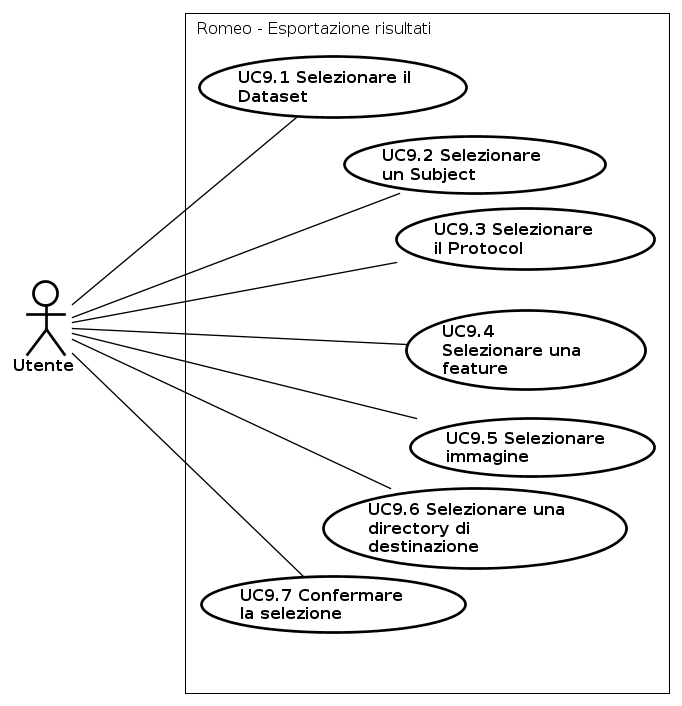
\includegraphics[scale=0.6]{./img/Use_Case/UC9}
\caption{UC9 - Esportazione risultati}
\end{center}
\end{figure}
\begin{itemize}
\item \textbf{Attori:} Utente;
\item \textbf{Scopo e descrizione:} l'utente vuole esportare i risultati di un'analisi già effettuata. In primo luogo, deve selezionare il Dataset\glossario{} in cui sono contenuti i Subject\glossario{} di cui vuole esportare i risultati. Successivamente può scegliere dei particolari Subject\glossario{} di cui vuole esportare i risultati, altrimenti verrà esportato l'intero gruppo. In secondo luogo, deve selezionare il Protocol\glossario{} interessato ed infine deve indicare la directory di destinazione dell'esportazione. I formati disponibili per l'esportazione sono: \verb|PNG|, \verb|BMP|, \verb|JPG|, NIfTI\glossario{} e Analyze7.5;
\item \textbf{Precondizione:} l'utente deve già aver effettuato un'analisi e deve aver deciso di esportare dei risultati;
\item \textbf{Flusso principale degli eventi:}
\begin{enumerate}
\item l'utente deve selezionare il Dataset\glossario{} [UC9.1];
\item l'utente può selezionare un Subject\glossario{} [UC9.2];
\item l'utente deve selezionare il Protocol\glossario{} di cui vuole esportare i risultati [UC9.3];
\item l'utente può selezionare una feature extractors\glossario{} [UC9.4];
\item l'utente seleziona l'immagine relativa alla selezione precedente che vuole esportare [UC9.5];
\item l'utente deve selezionare la directory in cui vuole siano esportati i risultati selezionati [UC9.6];
\item l'utente conferma la selezione e la directory precedentemente indicati [UC9.7].
\end{enumerate}
\item \textbf{Postcondizione:} il sistema ha esportato i risultati selezionati dall'utente nella directory indicata.
\end{itemize}

\subsection{Caso d'uso UC9.1: Selezione Dataset}
\begin{itemize}
\item \textbf{Attori:} Utente;
\item \textbf{Scopo e descrizione:} l'utente seleziona il Dataset\glossario{} in cui sono contenuti i risultati che vuole esportare;
\item \textbf{Precondizione:} il sistema mostra i Dataset\glossario{} memorizzati al suo interno;
\item \textbf{Flusso principale degli eventi:}
\begin{enumerate}
\item l'utente seleziona un Dataset\glossario{} di cui è già stata effettuata l'analisi. 
\end{enumerate}
\item \textbf{Postcondizione:} il sistema mostra i Subject\glossario{} presenti nel Dataset\glossario{} selezionato.
\end{itemize}

\subsection{Caso d'uso UC9.2: Selezionare un Subject}
\begin{itemize}
\item \textbf{Attori:} Utente;
\item \textbf{Scopo e descrizione:} l'utente seleziona un Subject\glossario{} di cui vuole esportare i risultati;
\item \textbf{Precondizione:} il sistema visualizza i Subject\glossario{} presenti nel Dataset\glossario{} precedentemente selezionato;
\item \textbf{Flusso principale degli eventi:}
\begin{enumerate}
\item l'utente seleziona un Subject\glossario{}.
\end{enumerate}
\item \textbf{Postcondizione:} il sistema evidenzia il Subject\glossario{} selezionato e sa di cui dovrà esportare i risultati.
\end{itemize}

\subsection{Caso d'uso UC9.3: Selezionare il Protocol}
\begin{itemize}
\item \textbf{Attori:} Utente;
\item \textbf{Scopo e descrizione:} l'utente seleziona il Protocol\glossario{} di cui vuole esportare i risultati;
\item \textbf{Precondizione:} il sistema visualizza i Protocol\glossario{} presenti nel Dataset\glossario{} precedentemente selezionato;
\item \textbf{Flusso principale degli eventi:}
\begin{enumerate}
\item l'utente seleziona un Protocol\glossario{}.
\end{enumerate}
\item \textbf{Postcondizione:} il sistema evidenzia il Protocol\glossario{} selezionato dall'utente.
\end{itemize}

\subsection{Caso d'uso UC9.4: Selezionare una feature extractor}
\begin{itemize}
\item \textbf{Attori:} Utente;
\item \textbf{Scopo e descrizione:} l'utente seleziona una feature extractor\glossario{} del quale vuole esportare il risultato;
\item \textbf{Precondizione:} il sistema visualizza le feature extractor\glossario{} presenti nel Protocol\glossario{} precedentemente selezionato;
\item \textbf{Flusso principale degli eventi:}
\begin{enumerate}
\item l'utente seleziona una feature extractor\glossario{}.
\end{enumerate}
\item \textbf{Postcondizione:} il sistema mostra le immagini relative alla feature extractor\glossario{} selezionata dall'utente.
\end{itemize}

\subsection{Caso d'uso UC9.5: Selezionare un immagine}
\begin{itemize}
\item \textbf{Attori:} Utente;
\item \textbf{Scopo e descrizione:} l'utente seleziona un'immagine del quale vuole esportare il risultato, relativa alla feature extractor\glossario{} precedentemente selezionata;
\item \textbf{Precondizione:} il sistema visualizza le immagini relative alla feature extractor\glossario{} precedentemente selezionata;
\item \textbf{Flusso principale degli eventi:}
\begin{enumerate}
\item l'utente seleziona un'immagine.
\end{enumerate}
\item \textbf{Postcondizione:} il sistema evidenzia l'immagine selezionata dall'utente.
\end{itemize}


\subsection{Caso d'uso UC9.6: Selezionare directory di destinazione}
\begin{itemize}
\item \textbf{Attori:} Utente;
\item \textbf{Scopo e descrizione:} l'utente deve scegliere la directory in cui vuole esportare i risultati;
\item \textbf{Precondizione:} il sistema attende che l'utente scelga la directory dove esportare i risultati;
\item \textbf{Flusso principale degli eventi:}
\begin{enumerate}
\item l'utente seleziona la directory in cui vuole esportare i risultati.
\end{enumerate}
\item \textbf{Postcondizione:} il sistema esporta i risultati desiderati dall'utente nella directory indicata.
\end{itemize}

\subsection{Caso d'uso UC9.7: Confermare la selezione}
\begin{itemize}
\item \textbf{Attori:} Utente;
\item \textbf{Scopo e descrizione:} l'utente conferma di voler esportare i risultati della selezione effettuata precedentemente;
\item \textbf{Precondizione:} l'utente ha selezionato gli elementi di cui vuole esportare i risultati;
\item \textbf{Flusso principale degli eventi:}
\begin{enumerate}
\item l'utente conferma di voler esportare i risultati relativi alla precedente selezione.
\end{enumerate}
\item \textbf{Postcondizione:} il sistema ha esportato i risultati richiesti dall'utente.
\end{itemize}

\pagebreak

\subsection{Caso d'uso UC10: Consultazione guida interattiva}
\begin{figure}[!h]
\begin{center}
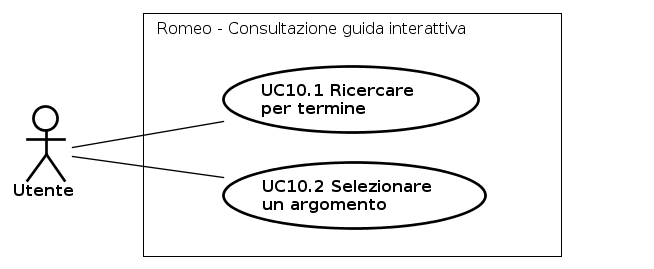
\includegraphics[scale=0.6]{./img/Use_Case/UC10}
\caption{UC10 - Consultazione guida interattiva}
\end{center}
\end{figure}
\begin{itemize}
\item \textbf{Attori:} Utente;
\item \textbf{Scopo e descrizione:} l'utente ha bisogno di un aiuto per utilizzare il software e può farlo in due modi: ricercando un termine nella guida, oppure scegliendo un argomento tra quelli proposti dal sistema. All'apertura della guida verranno comunque visualizzate informazioni riguardanti la funzione che l'utente sta svolgendo;
\item \textbf{Precondizione:} il sistema riceve la richiesta di aiuto dall'utente;
\item \textbf{Flusso generale degli eventi:}
\begin{enumerate}
\item l'utente può cercare un termine presente nella guida [UC10.1];
\item l'utente può selezionare un argomento proposto dalla guida [UC10.2].
\end{enumerate}
\item \textbf{Postcondizione:} il sistema ha mostrato le informazioni d'aiuto richieste dall'utente.
\end{itemize}

\subsection{Caso d'uso UC10.1: Ricercare per termine}
\begin{itemize}
\item \textbf{Attori:} Utente;
\item \textbf{Scopo e descrizione:} l'utente cerca un termine nella guida interattiva;
\item \textbf{Precondizione:} il sistema mostra la guida interattiva ed attende l'inserimento di un termine o la scelta di un argomento da parte dell'utente;
\item \textbf{Flusso principale degli eventi:}
\begin{enumerate}
\item l'utente effettua una ricerca inserendo un termine.
\end{enumerate}
\item \textbf{Postcondizione:} il sistema mostra le informazioni correlate al termine inserito dall'utente.
\end{itemize}

\subsection{Caso d'uso UC10.2: Selezionare un argomento}
\begin{itemize}
\item \textbf{Attori:} Utente;
\item \textbf{Scopo e descrizione:} l'utente seleziona un argomento fra quelli proposti dal sistema;
\item \textbf{Precondizione:} il sistema mostra la guida interattiva ed attende l'inserimento di un termine o la scelta di un argomento da parte dell'utente;
\item \textbf{Flusso principale degli eventi:}
\begin{enumerate}
\item l'utente seleziona un argomento tra quelli proposti.
\end{enumerate}
\item \textbf{Postcondizione:} il sistema mostra le informazioni correlate all'argomento selezionato dall'utente.
\end{itemize}

\subsection{Caso d'uso UC11: Eliminazione Dataset}
\begin{figure}[!h]
\begin{center}
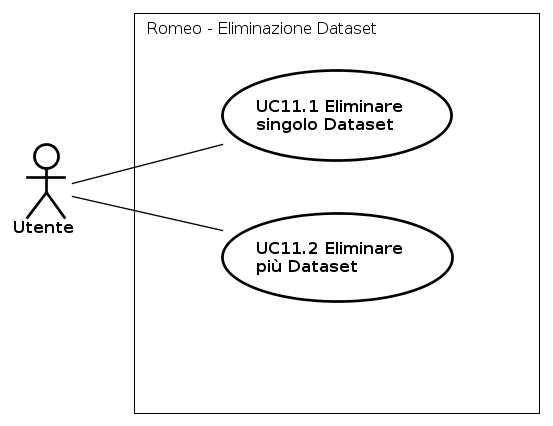
\includegraphics[scale=0.6]{./img/Use_Case/UC11}
\caption{UC11 - Eliminazione Dataset}
\end{center}
\end{figure}
\begin{itemize}
\item \textbf{Attore:} Utente;
\item \textbf{Scopo e descrizione:} l'utente può eliminare dei Dataset\glossario{} dal sistema e può farlo in due modi: eliminandone uno solo, oppure più di uno alla volta;
\item \textbf{Precondizione:} L'utente ha scelto di eliminare Dataset\glossario{}, nel sistema deve essere presente almeno un Dataset\glossario{};
\item \textbf{Flusso principale degli eventi:}
\begin{enumerate}
\item l'utente può eliminare un singolo Dataset\glossario{} [UC11.1];
\item l'utente può eliminare più Dataset\glossario{} [UC11.2].
\end{enumerate}
\item \textbf{Postcondizione:} il sistema ha eliminato i Dataset\glossario{} indicati dall'utente e i relativi risultati.
\end{itemize}

\pagebreak

\subsection{Caso d'uso UC11.1: Eliminare singolo Dataset}
\begin{figure}[!h]
\begin{center}
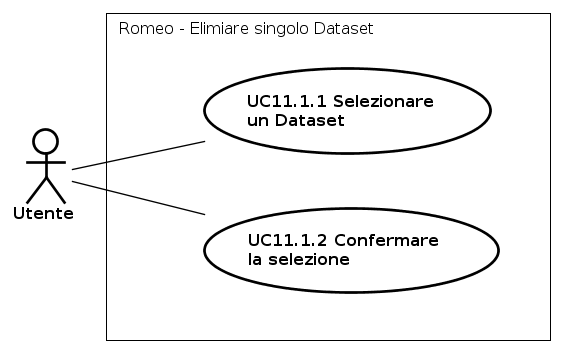
\includegraphics[scale=0.6]{./img/Use_Case/UC11_1}
\caption{UC11.1 - Eliminare singolo Dataset}
\end{center}
\end{figure}
\begin{itemize}
\item \textbf{Attore:} Utente;
\item \textbf{Scopo e descrizione:} l'utente seleziona il Dataset\glossario{} che intende eliminare e conferma la sua selezione;
\item \textbf{Precondizione:} l'utente ha scelto di eliminare un singolo Dataset\glossario{}, il sistema mostra l'elenco dei Dataset\glossario{} presenti nel sistema;
\item \textbf{Flusso principale degli eventi:}
\begin{enumerate}
\item l'utente seleziona il Dataset\glossario{} che desidera eliminare [UC11.1.1];
\item l'utente conferma di voler eliminare il Dataset\glossario{} selezionato [UC11.1.2].
\end{enumerate}
\item \textbf{Postcondizione:} il sistema ha eliminato il Dataset\glossario{} selezionato precedentemente dall'utente e ne ha rimosso i risultati;
\end{itemize}

\subsection{Caso d'uso UC11.1.1: Selezionare un Dataset}
\begin{itemize}
\item \textbf{Attore:} Utente;
\item \textbf{Scopo e descrizione:} l'utente seleziona un solo Dataset\glossario{} dalla lista proposta dal sistema;
\item \textbf{Precondizione:} il sistema mostra la lista dei Dataset\glossario{} presenti all'interno di esso;
\item \textbf{Flusso principale degli eventi:}
\begin{enumerate}
\item l'utente seleziona un solo Dataset\glossario{}.
\end{enumerate}
\item \textbf{Postcondizione:} il sistema evidenzia il Dataset\glossario{} selezionato dall'utente.
\end{itemize}

\subsection{Caso d'uso UC11.1.2: Confermare la selezione}
\begin{itemize}
\item \textbf{Attore:} Utente;
\item \textbf{Scopo e descrizione:} l'utente conferma di voler eliminare il Dataset\glossario{} precedentemente selezionato;
\item \textbf{Precondizione:} l'utente deve aver selezionato in precedenza un Dataset\glossario{};
\item \textbf{Flusso principale degli eventi:}
\begin{enumerate}
\item l'utente conferma l'eliminazione del Dataset\glossario{} evidenziato dal sistema.
\end{enumerate}
\item \textbf{Postcondizione:} il sistema ha eliminato il Dataset\glossario{} scelto dall'utente.
\end{itemize}


\subsection{Caso d'uso UC11.2: Eliminare singolo Dataset}
\begin{figure}[!h]
\begin{center}
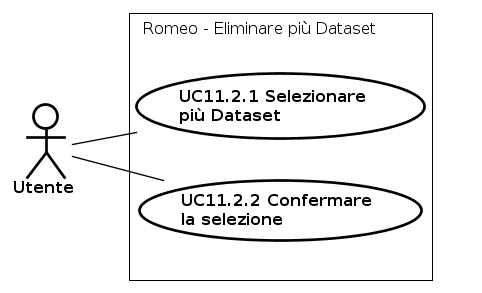
\includegraphics[scale=0.6]{./img/Use_Case/UC11_2}
\caption{UC11.2 - Eliminare più Dataset}
\end{center}
\end{figure}
\begin{itemize}
\item \textbf{Attore:} Utente;
\item \textbf{Scopo e descrizione:} l'utente seleziona i Dataset\glossario{} che intende eliminare e conferma la sua selezione;
\item \textbf{Precondizione:} l'utente ha scelto di eliminare più di un Dataset\glossario{}, il sistema mostra l'elenco dei Dataset\glossario{} presenti nel sistema;
\item \textbf{Flusso principale degli eventi:}
\begin{enumerate}
\item l'utente seleziona i Dataset\glossario{} che desidera eliminare [UC11.2.1];
\item l'utente conferma di voler eliminare i Dataset\glossario{} selezionati [UC11.2.2].
\end{enumerate}
\item \textbf{Postcondizione:} il sistema ha eliminato i Dataset\glossario{} selezionati precedentemente dall'utente e ne ha rimosso i risultati;
\end{itemize}

\subsection{Caso d'uso UC11.2.1: Selezionare più Dataset}
\begin{itemize}
\item \textbf{Attore:} Utente;
\item \textbf{Scopo e descrizione:} l'utente seleziona più di un Dataset\glossario{} dalla lista proposta dal sistema;
\item \textbf{Precondizione:} il sistema mostra la lista dei Dataset\glossario{} presenti all'interno di esso;
\item \textbf{Flusso principale degli eventi:}
\begin{enumerate}
\item l'utente seleziona più di un Dataset\glossario{}.
\end{enumerate}
\item \textbf{Postcondizione:} il sistema evidenzia i Dataset\glossario{} selezionati dall'utente.
\end{itemize}

\subsection{Caso d'uso UC11.2.2: Confermare la selezione}
\begin{itemize}
\item \textbf{Attore:} Utente;
\item \textbf{Scopo e descrizione:} l'utente conferma di voler eliminare i Dataset\glossario{} precedentemente selezionati;
\item \textbf{Precondizione:} l'utente deve aver selezionato in precedenza più di un Dataset\glossario{};
\item \textbf{Flusso principale degli eventi:}
\begin{enumerate}
\item l'utente conferma l'eliminazione dei Dataset\glossario{} evidenziati dal sistema.
\end{enumerate}
\item \textbf{Postcondizione:} il sistema ha eliminato i Dataset\glossario{} scelti dall'utente.
\end{itemize}